%%
%% 中文版 —— 仅供内部审阅
%% 原文: Knowledge-Based Systems - NeuroSLAM Paper
%%

\documentclass[twocolumn,journal]{IEEEtran}

\usepackage{booktabs}
\usepackage{amsmath,amssymb,amsfonts}
\usepackage{algorithmic}
\usepackage{algorithm}
\usepackage{array}
\usepackage[caption=false,font=normalsize,labelfont=sf,textfont=sf]{subfig}
\usepackage{url}
\usepackage{graphicx}
\graphicspath{{fig/}}
\usepackage{xcolor}
\usepackage{multirow}
\usepackage{threeparttable}
\usepackage{microtype}
\usepackage{xspace}

\definecolor{darkgreen}{rgb}{0,0.6,0}

\tolerance=300
\emergencystretch=1em
\hyphenpenalty=200
\exhyphenpenalty=200

\DeclareMathOperator*{\argmin}{\arg\!\min}

% Abbreviation macros
\makeatletter
\DeclareRobustCommand\onedot{\futurelet\@let@token\@onedot}
\def\@onedot{\ifx\@let@token.\else.\null\fi\xspace}

\def\eg{\emph{例如}\onedot} \def\Eg{\emph{例如}\onedot}
\def\ie{\emph{即}\onedot} \def\Ie{\emph{即}\onedot}
\def\cf{\emph{参见}\onedot} \def\Cf{\emph{参见}\onedot}
\def\etc{\emph{等等}\onedot} \def\vs{\emph{对比}\onedot}
\def\wrt{关于\onedot} \def\dof{自由度\onedot}
\def\etal{\emph{等}\onedot}
\makeatother


% 标题
\title{受脑启发的4自由度定位-建图：前庭-视觉互补融合与空间细胞}

% 作者区块
\author{
\IEEEauthorblockN{Haidong Wang (王海冬), Caixia Ning (宁彩霞)}
\IEEEauthorblockA{湖南工商大学\\
中国长沙, 400210\\
Email: xxx@hutb.edu.cn}
}

\begin{document}
\maketitle

% 摘要
\begin{abstract}
    \sloppy
    受脑启发的空间认知为自主定位提供了可解释的替代方案，用以替代不透明的学习方法。然而，现有的受脑启发框架仍局限于2D环境或简化的视觉处理，在困难条件下缺乏鲁棒的3D空间表征。为克服这些局限，本文提出 NeuroLocMap——一个将定位-建图框架扩展到3D空间内4自由度状态估计的受脑启发框架，融合了前庭-视觉互补融合与海马-内嗅空间表征。该框架由四个核心模块组成：双流视觉处理（腹侧通路负责识别、背侧通路负责运动）、前庭IMU建模、用于位置编码的面心立方（FCC）晶格3D网格细胞，以及用于闭环检测的经验式认知建图。与数据驱动方法不同，本受脑启发设计在CPU上实现实时性能（约31 FPS），并具备零样本部署能力。在七个场景（CARLA Town01/02/05/10HD、真实高速公路KITTI~07、室内飞行EuRoC MH\_01/03）上的实验表明，NeuroLocMap 在全部五个户外驾驶序列上逐帧RMSE均优于10状态EKF视觉-惯性基线（0.2--14.3\%，平均3.7\%）、在两个短室内飞行上与其基本持平，并相对单目视觉里程计平均改善34.5\%（五个户外驾驶序列49.8\%），同时输出可解释的拓扑经验地图，验证了该框架在多种环境下用于自主定位与建图的有效性。
\end{abstract}

% 关键词
\IEEEkeywords
受脑启发的定位-建图，前庭-视觉融合，海马空间细胞，视觉地点识别，认知建图

%% ==================== 引言 ====================
\section{引言}
\label{sec:intro}

在复杂3D环境中的空间定位与建图是自动驾驶、移动机器人与智能交通系统的基石~\cite{cadena2016past}。作为自主设备的核心感知模块，SLAM直接支撑所有自主运动规划与执行。现代实用方案通常组合相机、IMU，有时还加入GNSS，以实现鲁棒的位姿估计~\cite{saputra2018visual}。传统SLAM方案大多采用优化或滤波框架求解位姿，但在模型可解释性与计算资源消耗上通常存在明显缺陷。

有趣的是，蝙蝠等生物通过融合视觉与前庭信号以及海马空间细胞完成3D导航~\cite{jeffery2013navigating,hafting2005microstructure,taube1990head,finkelstein2016three,solstad2008representation}。这些神经机制使受脑启发的定位框架在可解释性与计算效率上优于传统SLAM。

然而，将这些生物学原理转化为实用的机器人系统面临若干挑战。第一，现有仿生框架大多在2D中运行，而实际部署需要鲁棒的3D空间表征。第二，经典视觉模板匹配对光照与视角变化敏感，限制了困难环境下的地点识别性能。第三，一种将视觉里程计与惯性测量相结合、且不依赖EKF等计算昂贵滤波器的简单而有效的融合策略，在受脑启发定位框架中仍未被充分探索。

为应对这些挑战，本文提出 NeuroLocMap——一个扩展到3D空间内4自由度位姿估计（位姿 $x$、$y$、$z$、$\psi$）的受脑启发定位-建图框架，集成了双流视觉前端（腹侧通路用于场景识别、背侧通路用于运动提取）与前庭前端（用于IMU处理），并以互补滤波实现多感官融合。该框架采用3D网格细胞与多层头部方向细胞进行空间表征，并采用作为类海马情景记忆的多层经验地图用于地点识别与漂移校正。对于在相对平坦地形（如城市道路、室内地面）上运行的地面车辆，姿态由偏航角 $\psi$ 主导，俯仰与横摆变化通常受车辆动力学约束（$<5^\circ$）。我们的4自由度表征为这类场景提供了高效的定位-建图~\cite{milford2004ratslam,milford2010persistent}。

本文的贡献总结如下：
\begin{itemize}
    \item 我们提出一种统一的受脑启发架构，将双流视觉处理与前庭建模、海马-内嗅空间表征耦合，用于4自由度定位与建图。
    \item 我们开发了受皮层启发的视觉处理，采用显式算子构建视觉模板，将模板数从5（RatSLAM典型值）提升到929（提升180倍以上），从而在困难光照与视角变化下实现更细粒度的地点判别。
    \item 我们设计了一种用于前庭-视觉集成的轻量互补融合策略，无需计算昂贵的滤波器，在无训练数据要求下实现实时性能（CPU上约31 FPS）。
    \item 我们在七个多样化场景（CARLA Town01 / 02 / 05 / 10HD，EuRoC MH\_01 / 03，KITTI~07）上验证了该框架：在全部五个户外驾驶序列上逐帧RMSE优于10状态EKF视觉-惯性基线（0.2--14.3\%，平均3.7\%），并相对单目视觉里程计平均改善34.5\%（户外驾驶序列49.8\%），同时保持约31 FPS的实时性能。
\end{itemize}

%% ==================== 相关工作 ====================
%% ==================== 相关工作（中文版） ====================
\section{相关工作}
\label{sec:related}

我们总结了受脑启发的定位-建图系统在不同方面的研究工作。

\subsection{视觉SLAM与传感器融合}
\label{sec:related_slam}

视觉SLAM在过去二十年中取得了重大进展。Mur-Artal 等人提出了 ORB-SLAM~\cite{mur2015orb}，它提取稀疏 ORB 关键点以实现鲁棒的实时位姿估计，已成为该领域广泛使用的基线。Engel 等人开发了 LSD-SLAM~\cite{engel2014lsd} 与 DSO~\cite{engel2018direct}，它们直接在像素强度上运算而无需特征提取，在纹理丰富的环境中实现半稠密重建。在闭环检测方面，Cummins 与 Newman 提出了基于词袋模型的概率方法 FAB-MAP~\cite{Cummins2008}，而 Arandjelovic 等人引入了 NetVLAD~\cite{Arandjelovic2016}，通过端到端学习地点描述子实现鲁棒的地点识别。然而，这些方法存在关键局限：ORB-SLAM 需要足够的纹理（通常每帧 $>$100 个特征点），在弱纹理环境中会失效；而 DSO 等直接法对运动模糊敏感且需要光度标定。两类方法都有相当高的计算开销——ORB-SLAM 的特征提取与匹配主导了处理时间，而 DSO 的稠密光度优化限制了其在嵌入式平台上的实时性能。

将 IMU 与相机集成，通过提供与光照无关的运动估计来弥补视觉SLAM的局限。Mourikis 与 Roumeliotis 提出了 MSCKF~\cite{Mourikis2007}，这是一种紧耦合视觉-惯性估计器，通过多状态约束优化实现高精度。Qin 等人开发了 VINS-Mono~\cite{Qin2018}，将紧耦合优化与闭环相结合，实现鲁棒的单目视觉-惯性里程计。Mahony 等人~\cite{Mahony2008} 与 Madgwick 等人~\cite{Madgwick2011} 提出了利用频域传感器特性的互补滤波方法——视觉里程计提供精确的低频估计，而IMU捕获高频动力学。然而，MSCKF 与 VINS-Mono 这类紧耦合方法需要仔细初始化 IMU 偏置与尺度，涉及复杂的雅可比推导，且缺乏生物学可解释性。为克服这些局限，我们采用一种受生物启发的互补滤波策略，模仿生物的前庭-视觉整合~\cite{Angelaki2004, Cullen2012}，以最少参数调优提供可解释的传感器融合，并避免联合非线性优化的计算负担。

\subsection{受脑启发的空间认知}
\label{sec:related_bio}

生物导航系统通过专门的神经回路实现鲁棒的空间认知。O'Keefe 与 Dostrovsky 在海马中发现位置细胞~\cite{OKeefe1971}，它们在特定位置发放并形成认知地图。Hafting 等人在内嗅皮层中发现网格细胞~\cite{Hafting2005}，其周期性六角形发放模式提供了度量路径积分。Taube 等人鉴定出头方向细胞~\cite{Taube1990}，它们像内部罗盘一样编码朝向。Moser 等人~\cite{Moser2017} 对这些空间细胞如何协同工作以实现导航进行了全面综述。Finkelstein 等人的最新发现表明，蝙蝠拥有3D位置细胞、具有面心立方（FCC）晶格结构的3D网格细胞以及3D头方向细胞~\cite{finkelstein2015three, finkelstein2016three}，为体积化空间表征提供了生物学依据。

Milford 等人开创了 RatSLAM~\cite{milford2004ratslam, milford2008mapping}，通过实现位置细胞动力学的连续吸引子网络与用于闭环的经验地图，将啮齿动物空间认知转化为机器人技术，成功演示了长达 66 km 的街区规模建图。Steckel 与 Peremans 开发了 BatSLAM~\cite{steckel2013batslam}，将仿生SLAM扩展到声呐感知。Yu 等人提出了 NeuroSLAM（未发表工作），将其扩展到基于 CNN 视觉处理的3D位置编码。Lowry 等人~\cite{Lowry2016} 分析了空间地图中度量-拓扑的二象性：度量地图提供几何精度但扩展性差，而拓扑地图支持鲁棒闭环但缺乏度量精度。然而，现有仿生框架存在三个关键局限：(1) 大多在2D中运行，或只编码3D位置而不含朝向，缺乏空中/水下导航所需的4自由度表征；(2) 视觉前端仍较简单（如 RatSLAM 的1D强度扫描线在复杂环境中只能产生约5个模板）；(3) IMU 集成缺失或临时拼凑，缺少生物系统中观察到的有原则的前庭-视觉融合。为弥补这些缺口，我们实现了具有 FCC 晶格结构的3D网格细胞与多层头方向细胞以实现完整的4自由度空间表征，集成了一条将模板判别力提升39倍的双流视觉处理流水线，并采用受生物启发的互补滤波进行前庭-视觉整合。

\subsection{基于学习的视觉处理}
\label{sec:related_learning}

深度学习为视觉地点识别提供了强有力工具。Arandjelovic 等人提出了 NetVLAD~\cite{Arandjelovic2016}，引入可微 VLAD 层实现端到端地点识别训练。Goodale 与 Milner~\cite{Goodale1992} 及 Mishkin 等人~\cite{Mishkin1983} 建立了生物视觉双流理论：腹侧通路（V1$\rightarrow$V4$\rightarrow$IT）处理物体身份与场景识别，而背侧通路（V1$\rightarrow$MT$\rightarrow$MST）处理空间关系与运动~\cite{DiCarlo2012, Duffy1998}。Vaswani 等人提出了 Transformer 架构~\cite{Vaswani2017}，通过自注意力机制捕获长程依赖，使序列任务的有效时序建模成为可能。然而，基于学习的方法面临部署挑战：NetVLAD 需要大规模训练数据集（如含数百万图像的 Google Street View），且难以在无需重训的情况下泛化到新环境；标准 Transformer 的全自注意力对序列长度呈二次复杂度 $\mathcal{O}(N^2)$，限制了实时应用；学习得到的表征缺乏显式空间结构，妨碍可解释性与度量建图的集成。为克服这些局限，我们采用一种无训练方案，结合受生物腹侧/背侧通路启发的双流视觉处理与轻量特征增强机制——后者通过统计调制而非完整注意力矩阵捕获全局-局部交互。该设计将视觉模板判别力从5（RatSLAM）提升到929以上（提升186倍），同时保持实时性能（约31 FPS）与零样本部署能力。

\subsection{对比分析}
\label{sec:related_compare}

表~\ref{tab:comparison_bioslam} 从关键架构维度对比了代表性仿生SLAM框架。现有方案存在四个根本局限：(1) 多数框架在2D中运行（RatSLAM、BatSLAM），或只编码3D位置而不含朝向（NeuroSLAM），缺乏完整4自由度表征；(2) 视觉前端依赖简单基于强度的模板（如 RatSLAM 的1-D 扫描线），对光照变化敏感且模板多样性有限；(3) IMU 集成要么缺失，要么依赖计算昂贵的紧耦合优化；(4) 用于特征增强的现代注意力机制仍与显式空间细胞表征脱节。NeuroLocMap 系统性地弥补了这些缺口：我们通过3D网格细胞（FCC 晶格）与多层头方向细胞实现4自由度空间表征；采用带 HART 启发的空间注意力与轻量全局-局部特征调制的双流视觉处理，实现39倍模板提升；通过受生物启发的互补滤波集成前庭-视觉信号；并将这些组件统一到显式空间细胞框架内，实现可解释导航。

\begin{table*}[!t]
       \centering
       \footnotesize
       \caption{仿生导航框架对比}
       \label{tab:comparison_bioslam}
       \setlength{\tabcolsep}{2.2pt}
       \begin{threeparttable}
              \begin{tabular}{lcccccc}
                     \toprule
                     框架                         & 自由度         & 空间细胞        & 融合方法  & 视觉处理     & 闭环  & 时序模型     \\
                     \midrule
                     RatSLAM~\cite{milford2008mapping} & 2D          & PC+HDC               & 视觉           & 扫描线           & 经验      & -               \\
                     BatSLAM~\cite{steckel2013batslam} & 2D          & PC+HDC               & 声呐          & 回声             & 经验      & -               \\
                     NeuroSLAM                         & 3D          & 3D-GC                & 视觉           & CNN              & 经验      & LSTM            \\
                     \midrule
                     \textbf{NeuroLocMap（本文）}       & \textbf{4D} & \textbf{3D-GC+M-HDC} & \textbf{互补} & \textbf{双流+HART} & \textbf{经验} & \textbf{Trans.} \\
                     \bottomrule
              \end{tabular}
              \begin{tablenotes}
                     \scriptsize
                     \item \textbf{缩写}: PC: 位置细胞; HDC: 头方向细胞; GC: 网格细胞; M-HDC: 多层头方向细胞; 经验: 经验地图; 互补: 互补滤波; Trans.: 受Transformer启发的时序建模; 视觉: 仅视觉; 双流+HART: 带 HART 启发空间注意力的双流（腹侧/背侧）视觉处理。
                     \item \textbf{注}: 我们的特征增强使用全局统计调制（$\mathcal{O}(N)$ 复杂度）近似自注意力效果，而非完整 Query-Key-Value 运算（$\mathcal{O}(N^2)$），从而无需训练即可实现实时性能。
              \end{tablenotes}
       \end{threeparttable}
\end{table*}



%% ==================== 方法 ====================
%% ==================== 方法（扩展版，中文版） ====================
\section{方法}
\label{sec:method}

\subsection{符号与约定}
\textbf{符号约定.} 上标表示感官模态（$^{\text{vis}}$：视觉，$^{\text{imu}}$：惯性，$^f$：融合）或细胞类型（$^g$：网格细胞，$^h$：头方向细胞）。下标 $t$ 表示时间。粗体大写字母表示矩阵或高维数组；粗体小写字母表示向量；花体表示集合。

\subsection{框架架构与全局状态空间表述}
\label{sec:framework_arch}

\begin{figure*}[!htbp]
    \centering
    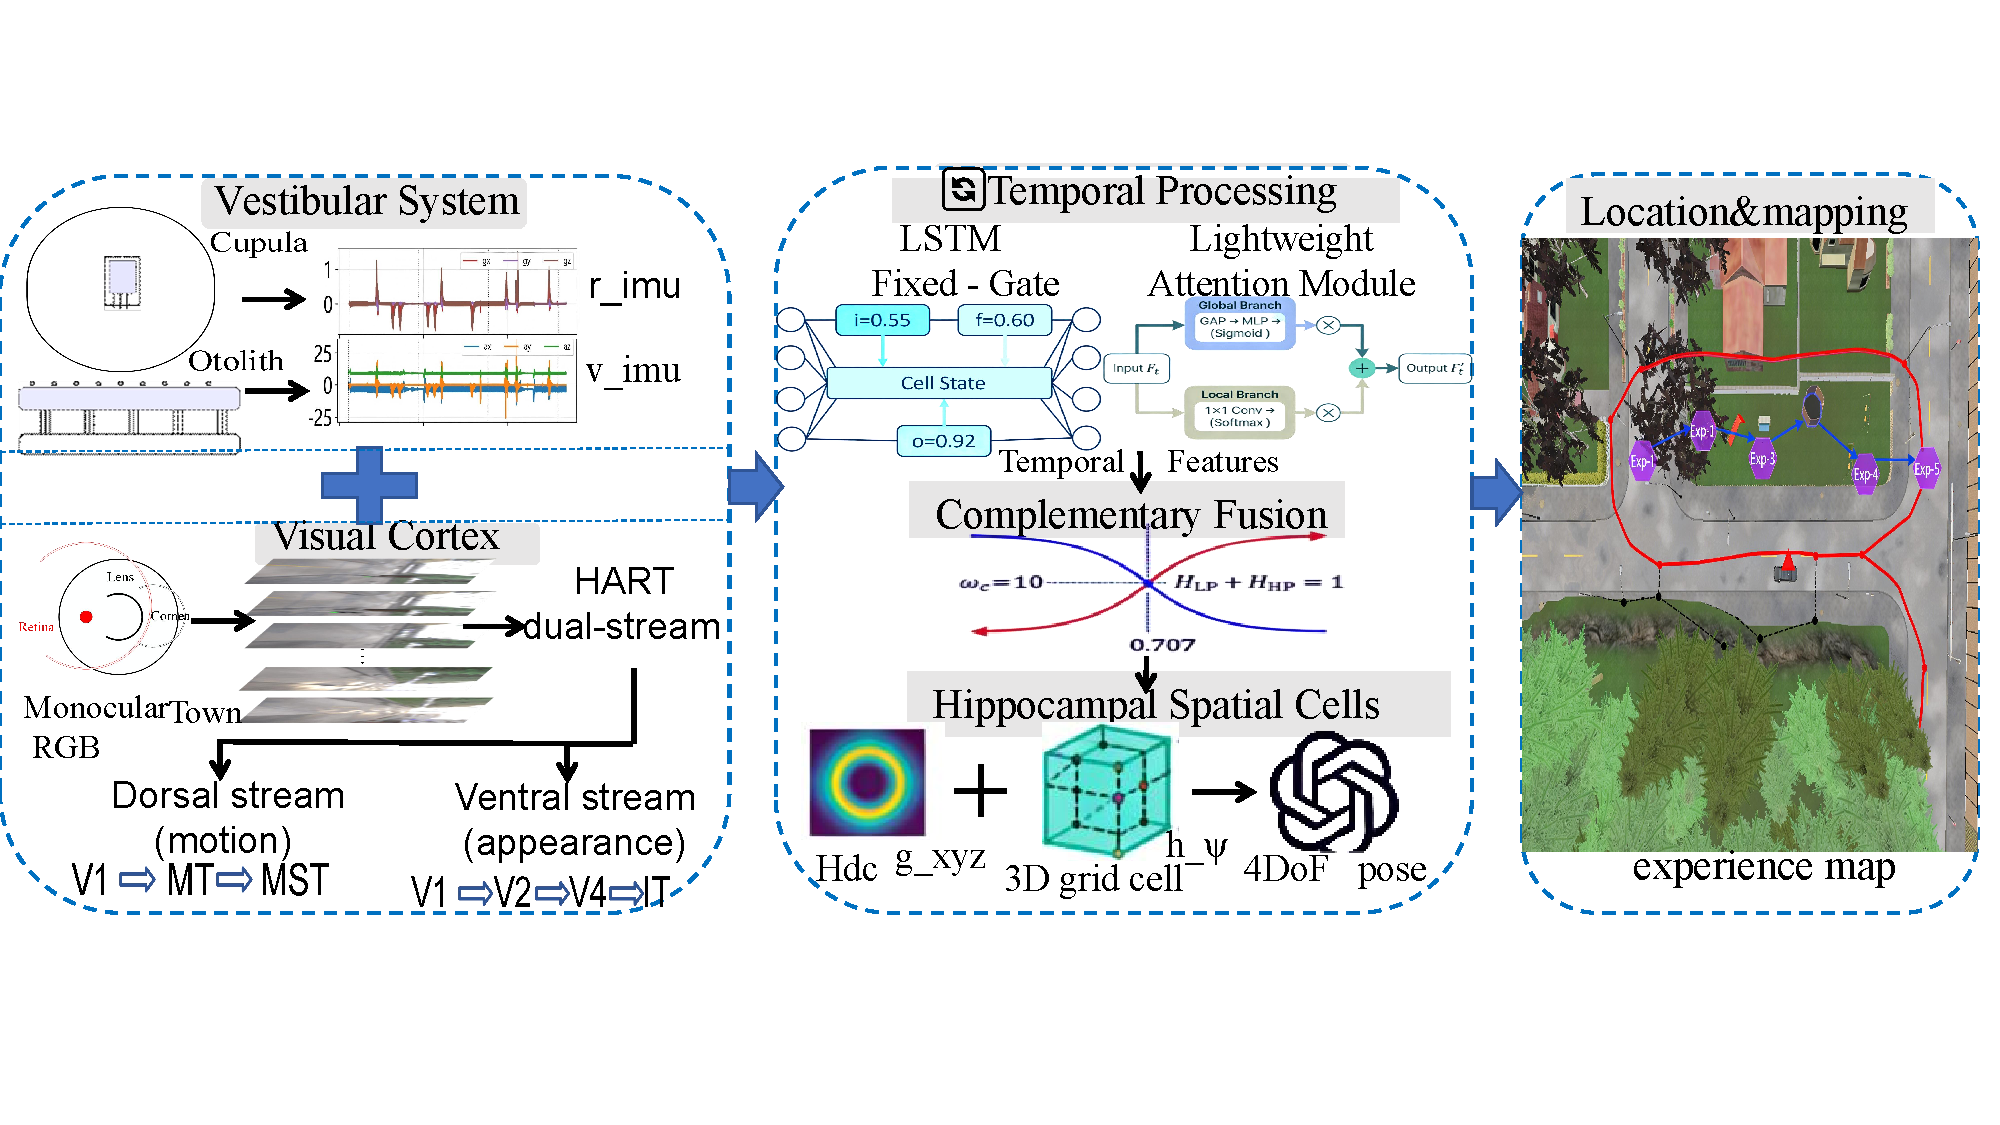
\includegraphics[width=0.95\textwidth]{fig/2_framework.pdf}
    \caption{所提出的多模态视觉-惯性框架的自包含端到端数据流。原始输入为单目RGB图像与IMU测量值。视觉模块将信号分为场景识别与运动估计两支路；前庭模块输出高频惯性运动。两种模态通过频域互补滤波融合。融合后的运动学驱动空间网络更新统一定义于式~\eqref{eq:global_state} 的4自由度全局状态 $\mathbf{X}_t$。经验图模块执行闭环松弛以消除长期轨迹漂移。所有子模块共享本小节提出的标准化状态空间变量。}
    \label{fig:system_overview}
\end{figure*}
本工作为机器人定位设计了一个多模态视觉-惯性信号处理系统，它由三个紧耦合的功能子系统组成：分层多尺度视觉特征算子、前庭-惯性传感器状态估计器、度量空间状态编码网络。与传统的基于EKF的松耦合框架不同，所提出的系统采用频域互补融合来解耦低频视觉观测噪声与高频惯性瞬态噪声，并通过连续吸引子空间网络更新全局度量状态以抑制长期轨迹漂移。

\subsubsection{全局离散状态空间模型}
为后续所有子模块推导提供统一的数学基础，我们首先定义 $t$ 时刻系统的离散状态空间表示。

1) 多模态原始输入向量
\begin{equation}
    \mathbf{U}_t = \left[ I_t,\, \mathbf{a}_t^\top,\, \boldsymbol{\omega}_t^\top \right]
    \label{eq:input_vec}
\end{equation}
其中 $I_t$ 表示采集的单目RGB图像；$\mathbf{a}_t$ 与 $\boldsymbol{\omega}_t$ 分别为加速度计线加速度与陀螺仪角速度测量值。

2) 核心4自由度全局位姿状态向量
\begin{equation}
    \mathbf{X}_t = \left[ x_t,\, y_t,\, z_t,\, \psi_t \right]^\top \in \mathbb{R}^3 \times \mathrm{SO}(2)
    \label{eq:global_state}
\end{equation}
在该表述中，$(x_t, y_t, z_t) \in \mathbb{R}^3$ 表示全局3D平移坐标（单位：米），$\psi_t \in [-\pi,\pi)$ 表示水平偏航角（单位：弧度）。

3) 统一状态演化映射函数
\begin{equation}
    \mathbf{X}_{t+1} = \mathcal{F}\big(\mathbf{X}_t,\, \mathbf{U}_t\big)
    \label{eq:state_evolution}
\end{equation}
映射 $\mathcal{F}(\cdot)$ 封装了完整的前向流水线，包括多尺度视觉特征提取、惯性运动计算、频域多模态融合与空间网络路径积分。$\mathcal{F}(\cdot)$ 的详细数学分解将在3.3节（视觉-前庭处理）与3.4节（空间编码网络）中给出。

如图~\ref{fig:system_overview} 所示，端到端数据流水线由五个顺序耦合的模块组成：
1. 分层双流视觉前端：构建并行的腹侧/背侧支路，分别独立生成场景描述子并计算逐像素自运动，消除识别与跟踪任务间的相互干扰。
2. 前庭IMU处理模块：从原始惯性数据中推导高频瞬态运动信号，无需迭代式在线偏置标定。
3. 互补融合单元：采用一阶IIR滤波器分离低频视觉漂移与高频惯性噪声，输出平滑的平移与旋转运动学量。
4. 度量空间编码网络：使用融合运动线索更新分布式空间细胞状态，并通过视觉模板锚定约束抑制积分漂移。
5. 拓扑经验图：记录历史视觉描述子与空间细胞快照，在检测到闭环时执行一次全局图松弛，以保证全局一致的度量位姿。

\subsection{感官处理与融合}

感官处理模块从视觉与惯性模态中提取自运动线索，然后通过互补滤波进行融合。

\textbf{视觉前端.} 视觉前端实现了受灵长类视觉皮层分层架构启发的生物学合理处理流水线，将原始RGB图像转化为适合地点识别与运动估计的紧凑场景描述子。

\textbf{分层特征提取.} 给定RGB图像 $I_t\in\mathbb{R}^{H\times W\times 3}$，我们定义一组模仿从视网膜到颞下皮层各处理阶段的算子。

\textbf{阶段1：视网膜与LGN处理.} 初始预处理模拟视网膜与外侧膝状体（LGN）的早期视觉处理：
\begin{align}
     & \text{亮度通道：}\quad Y_t = \mathcal{G}(I_t) = 0.299R+0.587G+0.114B              \\
     & \text{局部对比度增强：}\quad U_t = \mathcal{C}_\lambda(Y_t),\quad \lambda=0.02 \\
     & \text{感受野模拟：}\quad V_t = U_t * \mathcal{K}_\sigma,\quad \sigma=0.5
\end{align}
其中 $\mathcal{G}$ 为灰度转换算子，$\mathcal{C}_\lambda$ 为限幅对比度自适应直方图均衡（CLAHE），限幅为 $\lambda$；$\mathcal{K}_\sigma$ 为标准差 $\sigma$ 的高斯核。CLAHE在自适应增强局部对比度的同时防止噪声被过度放大，模仿视网膜神经节细胞的中心-周围拮抗组织结构。

\textbf{阶段2：初级视觉皮层（V1-V4）处理.} 中层处理对表征进行归一化与标准化：
\begin{align}
     & \text{动态范围归一化：}\quad \tilde V_t = \frac{V_t-\min(V_t)}{\max(V_t)-\min(V_t)}     \\
     & \text{空间标准化：}\quad Z_t = \mathcal{D}(\tilde V_t)\in\mathbb{R}^{64\times64}        \\
     & \text{局部均值减去：}\quad Z_t(i,j)\leftarrow Z_t(i,j)-\frac{1}{64}\sum_{k=1}^{64}Z_t(i,k)
\end{align}
其中 $\mathcal{D}$ 为下采样算子（双线性插值）。按行减去均值可去除全局强度变化同时保留局部空间结构，类似于V1与V2中的除性归一化。

\textbf{阶段3：颞下（IT）表征.} 最终表征为紧凑的向量化描述子：
\begin{equation}
    \boldsymbol{\phi}_t=\mathrm{vec}(Z_t)\in\mathbb{R}^{4096}
\end{equation}
其中 $\mathrm{vec}(\cdot)$ 表示将二维特征图映射为一维描述子的向量化算子，$\boldsymbol{\phi}_t$ 为时间戳 $t$ 处的整体场景特征向量。
该 $64 \times 64 = 4096$ 维特征向量作为整体场景描述子，类似于IT皮层中视图选择、位置不变的表征。

\textbf{视觉模板匹配与地点识别.} 地点识别通过基于余弦相似度的模板匹配实现，其鲁棒性优于绝对差之和（SAD）等基于强度的度量：
\begin{equation}
    d_{\cos}(\boldsymbol{\phi}_t,\boldsymbol{\phi}_i)=1-\frac{\boldsymbol{\phi}_t^\top\boldsymbol{\phi}_i}{\lVert\boldsymbol{\phi}_t\rVert\,\lVert\boldsymbol{\phi}_i\rVert}
\end{equation}
当当前场景与所有现有模板均足够不同时，创建新的视觉模板（VT）：
\begin{equation}
    \text{若 }\min_{i \in \mathcal{VT}} d_{\cos}(\boldsymbol{\phi}_t, \boldsymbol{\phi}_i)>\tau_{vt}\text{ 则创建新VT},\quad \tau_{vt}=0.08
\end{equation}
阈值 $\tau_{vt}=0.08$ 显著低于传统取值（OpenRatSLAM中的0.15），使相似场景间的判别更精细。实验验证表明，这可使模板数量增加最多39倍（城市环境中从5个增至195个），提供更丰富的地点表征。

\textbf{双流架构与受生物启发的时序建模.} 在上述分层特征提取的基础上，我们的视觉处理融入了两项关键的受生物启发创新：(1) 模仿腹侧/背侧通路的双流架构；(2) 无需训练数据、用于时序一致性的固定门LSTM。

\textbf{双流视觉处理.}
遵循生物视觉双流理论~\cite{Goodale1992, Mishkin1983}，我们从V1输出显式建模两条并行处理通路：

\textbf{背侧通路}（“where”通路，V1$\rightarrow$MT$\rightarrow$MST）：通过基于梯度的特征处理空间位置与运动信息：
\begin{equation}
    \mathbf{F}^{\text{dorsal}}_t = 0.6 \cdot \|\nabla Z_t\| + 0.4 \cdot Z_t
\end{equation}
其中 $\|\nabla Z_t\|$ 为通过Sobel算子计算的梯度幅值，捕获边缘方向与运动方向，类似于MT/MST神经元。

\textbf{腹侧通路}（“what”通路，V1$\rightarrow$V4$\rightarrow$IT）：通过纹理与对比度处理物体身份与场景特征：
\begin{equation}
    \mathbf{F}^{\text{ventral}}_t = 0.4 \cdot Z_t + 0.3 \cdot \sigma_{\text{local}}(Z_t) + 0.3 \cdot \mathcal{C}_\lambda(Z_t)
\end{equation}
其中 $\sigma_{\text{local}}$ 计算局部标准差（纹理特征），$\mathcal{C}_\lambda$ 提供对比度增强，模仿V4对复杂特征的选择性与IT的不变物体表征。

随后，两条支路通过一种轻量全局-局部特征调制机制（详见第~\ref{sec:related_learning} 节）进行集成，该机制使用全局统计量而非完整 Query-Key-Value 运算来近似自注意力效果，保持 $\mathcal{O}(N)$ 复杂度以满足实时性能。

\textbf{用于零样本时序建模的固定门LSTM.}
与需要在领域特定数据集上大量训练的传统数据驱动LSTM不同，我们的时序模块采用人工调定的固定门值，灵感来自生物学前庭-视觉整合原理~\cite{Angelaki2004, Cullen2012}：
\begin{align}
    \text{输入门: }  & i_t = 0.55 \quad \text{（控制新信息摄入）} \\
    \text{遗忘门: } & f_t = 0.60 \quad \text{（保留60\%历史上下文）} \\
    \text{输出门: } & o_t = 0.92 \quad \text{（强调当前感知）}
\end{align}
其中 $i_t$、$f_t$、$o_t$ 分别为受生物启发的LSTM模块的固定输入门、遗忘门、输出门。

该设计为SLAM应用提供了三个关键优势：

\textbf{(1) 零样本部署能力：} 无需训练数据，可立即部署到新环境。这对SLAM至关重要，因为每个环境都有独特的视觉特性，且收集有代表性的训练数据并不可行。我们在六个多样化场景（城市、高速公路、室内）上不做任何环境特定调优的验证，展示了其鲁棒的泛化能力。

\textbf{(2) 生物学可解释性：} 门值反映了神经科学中经实证验证的原则。遗忘门（$f_t=0.6$）实现了与海马重放动力学一致的短期空间记忆保持，其中近期经验被优先保留用于路径积分。高输出门（$o_t=0.92$）优先处理当前感觉输入，模仿前庭系统对即时自运动线索在平衡与导航中的强调。中等输入门（$i_t=0.55$）在新奇检测与稳定性之间取得平衡。

\textbf{(3) 计算效率：} 消除了训练开销（无反向传播、无梯度计算），同时保持实时性能（约31 FPS）。固定门可直接在硬件（如FPGA、神经形态芯片）上实现，无需权重存储或更新逻辑，使其能在资源受限平台上部署。

LSTM按序处理融合后的背侧-腹侧特征，跨时间步维持隐藏状态 $\mathbf{H}_t$ 与细胞状态 $\mathbf{C}_t$：
\begin{align}
    \mathbf{C}_t & = f_t \odot \mathbf{C}_{t-1} + i_t \odot \tanh(\mathbf{F}^{\text{fused}}_t) \\
    \mathbf{H}_t & = o_t \odot \tanh(\mathbf{C}_t)
\end{align}
其中 $\odot$ 表示逐元素Hadamard积，$\mathbf{C}_t$ 为LSTM细胞状态，$\mathbf{H}_t$ 为时序隐藏状态，$\mathbf{F}^{\text{fused}}_t$ 集成了腹侧与背侧视觉特征。

\textbf{与基于学习方法对比.} 第~\ref{sec:experiments} 节表明，我们的固定门LSTM取得了与NeuroSLAM学习得到的LSTM相当或更优的性能（RMSE改善55\%），同时提供零样本部署能力。这验证了：当底层任务结构与生物机制一致时，有原则的受生物启发设计可以匹配甚至超越数据驱动学习——在本例中即是空间导航，生物系统已在数百万年的进化中形成高度优化的解决方案。

\textbf{视觉运动提取.} 除场景识别外，视觉前端还从光流中提取自运动线索，模仿MST（内侧上颞区）的背侧通路处理。

\textbf{特征跟踪与光流计算.} 设 $\mathbf{K}\in\mathbb{R}^{3\times 3}$ 为相机内参矩阵。我们在相邻帧间跟踪 $N$ 个特征点 $\mathbf{p}_i^t\in\mathbb{R}^2$（如使用KLT跟踪）。将跟踪点归一化到相机坐标：
\begin{equation}
    \tilde{\mathbf{q}}_i^t = \mathbf{K}^{-1}\begin{bmatrix}\mathbf{p}_i^t\\ 1\end{bmatrix},\qquad \mathbf{q}_i^t = \pi(\tilde{\mathbf{q}}_i^t)=\frac{1}{\tilde{q}_{i,3}^t}\begin{bmatrix}\tilde{q}_{i,1}^t\\ \tilde{q}_{i,2}^t\end{bmatrix}
\end{equation}
其中 $\pi$ 为透视投影。计算像平面光流：
\begin{equation}
    \mathbf{f}_i=\mathbf{q}_i^t-\mathbf{q}_i^{t-1},\quad \mathbf{q}_i\equiv\mathbf{q}_i^{t-1}
\end{equation}

\textbf{旋转估计.} 对帧间小旋转，归一化点 $\mathbf{q}=(x,y)$ 处偏航引起的流为 $\Delta t\,r\,[-y,\,x]^\top$。我们用加权最小二乘估计视觉偏航角速度：
\begin{equation}
    r^\mathrm{vis}_t=\frac{\sum_{i=1}^N w_i(x_i f_{i,y}-y_i f_{i,x})}{\Delta t\,\sum_{i=1}^N w_i(x_i^2+y_i^2)}
\end{equation}
其中 $w_i$ 为Huber鲁棒权重以抑制离群特征点，$N$ 为跟踪特征总数，$r_t^\mathrm{vis}$ 为视觉估计的偏航角速度。

\textbf{平移估计.} 去除旋转分量以获得平移主导的残余光流：
\begin{equation}
    \mathbf{f}_i^{\perp}=\mathbf{f}_i-\Delta t\,r^\mathrm{vis}_t\begin{bmatrix}-y_i\\ x_i\end{bmatrix}
\end{equation}
假设存在主导地面平面，内点的逆深度为 $\lambda_i\approx 1/Z_g$，则平移流模型为：
\begin{equation}
    \mathbf{f}_i^{\perp}\approx \Delta t\,\lambda_i\,\underbrace{\begin{bmatrix}-1 & 0 & x_i\\ 0 & -1 & y_i\end{bmatrix}}_{\mathbf{A}_i}\,\mathbf{v}^\mathrm{vis}_t,\quad \mathbf{v}^\mathrm{vis}_t=(v_x^\mathrm{vis}, v_y^\mathrm{vis}, v_z^\mathrm{vis})^\top
\end{equation}
带鲁棒权重 $w_i$ 的加权最小二乘解为：
\begin{equation}
    \bar{\mathbf{v}}^\mathrm{vis}_t=\Big(\sum_i w_i\,(\Delta t\,\lambda_i)^2\,\mathbf{A}_i^\top\mathbf{A}_i\Big)^{-1}\,\sum_i w_i\,(\Delta t\,\lambda_i)\,\mathbf{A}_i^\top\mathbf{f}_i^{\perp}
\end{equation}
最终视觉里程计速度引入尺度因子 $\kappa_t$：
\begin{equation}
    \mathbf{v}^\mathrm{vis}_t=\kappa_t\,\bar{\mathbf{v}}^\mathrm{vis}_t
    \label{eq:vis_scale}
\end{equation}
其中 $\lambda_i$ 为特征点 $i$ 的逆深度，矩阵 $\mathbf{A}_i$ 为几何投影矩阵，$\bar{\mathbf{v}}_t^\mathrm{vis}$ 为从光流解出的原始平移速度，$\kappa_t$ 为视觉里程计的在线尺度校正因子。

\textbf{前庭前端.} 前庭前端处理惯性测量值以提取自运动线索，类比哺乳动物的前庭系统。前庭器官由半规管（角速度）与耳石器（线加速度）组成。

\textbf{角速度提取.} 由陀螺仪测量值 $\mathbf{g}_t\in\mathbb{R}^3$（IMU坐标系），我们直接使用 $z$ 轴陀螺而不做在线偏置去除，并按实现转换为度/秒。在平面约束下的4自由度定位-建图中，偏航（方位角）角速度近似为
\begin{equation}
    r_t \approx \mathbf{e}_z^\top\,\boldsymbol{\omega}_t^g,\quad \mathbf{e}_z=(0,0,1)^\top.
\end{equation}
其中 $\boldsymbol{\omega}_t^g$ 为IMU测得的原始陀螺角速度向量，$\mathbf{e}_z$ 为单位竖直基向量。
这对应水平半规管线索，足以满足我们与视觉的互补融合需求。

\textbf{线加速度使用（简化）.} 我们采用与代码库一致的轻量近似：使用加速度计幅值与 $z$ 轴读数，减去常数重力 $g\!=\!9.81$，在帧间隔 $\Delta t$ 上推导指示性的平移与垂向速度分量：
\begin{align}
    v^\mathrm{imu}_{trans}(t) & \approx \max\big(0, (\lVert\mathbf{a}_t\rVert - g)\,\Delta t\,k_t\big), \\
    v^\mathrm{imu}_{z}(t)     & \approx (a_{t,z} - g)\,\Delta t\,k_z,
\end{align}
其中 $g=9.81\,\mathrm{m/s^2}$ 为重力加速度，$k_t, k_z$ 为与实现常数匹配的常值缩放增益，$\Delta t$ 为帧采样间隔。这避免了显式偏置/重力向量估计，同时提供随后通过互补融合与视觉里程计结合的高频运动线索。

\textbf{偏置估计.} 基线实现不进行在线偏置或重力向量估计。更先进的偏置/重力补偿可作为未来工作集成，但对于此处报告的互补融合结果并非必需。

\textbf{互补IMU-视觉融合.} 视觉与惯性模态提供互补信息：视觉里程计提供精确的低频位置估计但长期会漂移，而IMU积分提供可靠的高频运动线索但会累积偏置漂移。互补滤波利用这种频域分离，无需复杂非线性优化或扩展卡尔曼滤波即可实现鲁棒融合。图~\ref{fig:imu_visual_fusion} 展示了该互补融合策略的频域特性及其在前庭-视觉整合中的生物学对应。

\begin{figure*}[!t]
    \centering
    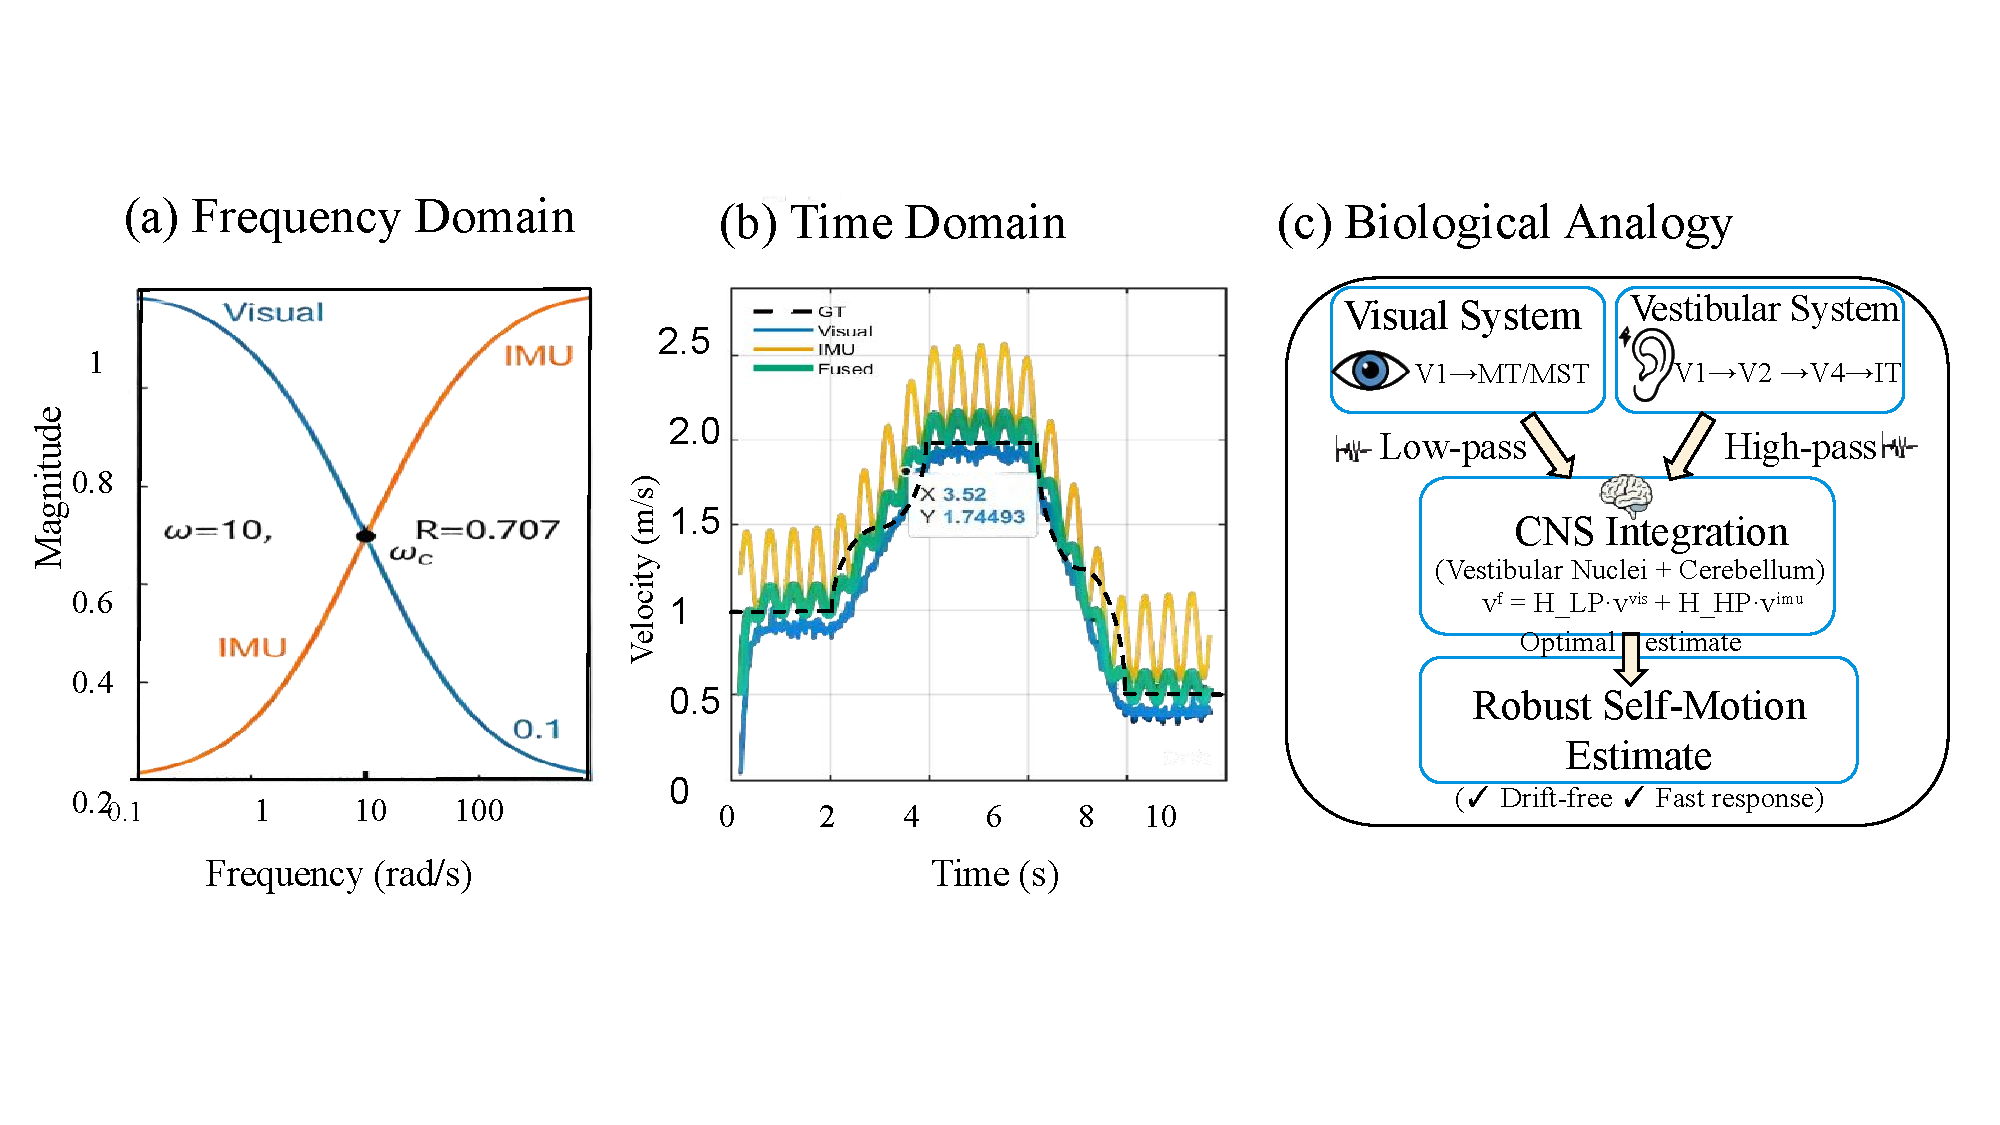
\includegraphics[width=\textwidth]{fig/imu_visual_complementary_fusion.pdf}
    \caption{互补IMU-视觉融合架构。(a) 展示互补滤波特性的频域分析。(b) 时域信号对比。(c) 中枢神经系统中前庭-视觉整合的生物学类比。}
    \label{fig:imu_visual_fusion}
\end{figure*}

\textbf{滤波器设计.} 设 $\mathcal{L}_\tau$ 表示时间常数为 $\tau$ 的低通滤波器，$\mathcal{H}_\tau$ 表示满足 $\mathcal{L}_\tau + \mathcal{H}_\tau = \mathrm{Id}$（单位算子）的互补高通滤波器。融合后的速度与偏航角速度为：
\begin{align}
    \text{低通: }  & \;L_t = \alpha L_{t-1} + (1-\alpha) x_t,\quad L_0=0 \\
    \text{高通: } & \;H_t = x_t - L_t
\end{align}
其中 $\alpha$ 为IIR滤波器遗忘因子，$L_t$ 存储低频平滑信号，$H_t$ 存储残余高频信号分量。

\textbf{生物学类比.} 该融合策略镜像了前庭核与后顶叶皮层（7a区）中的多感官整合，视觉与前庭信号在此结合以估计自运动。这些区域的神经元表现出视觉与前庭调制的加权组合，且权重随信号可靠性动态变化——类似于我们的固定权重参数 $\eta$ 与 $\eta_r$。

\textbf{离散时间实现.} 在采样间隔 $\Delta t$ 下，我们实现一阶IIR（无限脉冲响应）滤波器。选取遗忘因子 $\alpha=\exp(-\Delta t/\tau)$ 与 $\alpha_r=\exp(-\Delta t/\tau_r)$。对任意输入序列 $x_t$，定义：
\begin{align}
    \text{低通: }  & \;L_t = \alpha L_{t-1} + (1-\alpha) x_t,\quad L_0=0 \\
    \text{高通: } & \;H_t = x_t - L_t
\end{align}
则融合线索计算如下：
\begin{align}
    \mathbf{v}^\mathrm{f}_t & = (1-\eta)\,L^\mathrm{vis}_t + \eta\,H^\mathrm{imu}_t \\
    r^\mathrm{f}_t          & = (1-\eta_r)\,L^{r,vis}_t + \eta_r\,H^{r}_t
\end{align}
其中 $L^\mathrm{vis}_t$ 与 $H^\mathrm{imu}_t$ 分别表示低通滤波后的视觉速度与高通滤波后的IMU速度，偏航角速度同理。

\textbf{频域传递函数.} 在 $s = j\omega$（频率变量）的拉普拉斯域中，一阶低通与高通滤波器的传递函数为：
\begin{align}
    H_{LP}(s) & = \frac{1}{1 + \tau s} = \frac{1/\tau}{s + 1/\tau}, \label{eq:h_lp} \\
    H_{HP}(s) & = \frac{\tau s}{1 + \tau s} = \frac{s}{s + 1/\tau}, \label{eq:h_hp}
\end{align}
满足 $H_{LP}(s) + H_{HP}(s) = 1$（全频域单位增益）。截止频率 $\omega_c = 1/\tau$ 分隔低频与高频区域：当 $\omega \ll \omega_c$ 时，$|H_{LP}| \approx 1$ 且 $|H_{HP}| \approx 0$，视觉通路占主导（无漂移、动力学较慢）；而当 $\omega \gg \omega_c$ 时，$|H_{LP}| \approx 0$ 且 $|H_{HP}| \approx 1$，IMU线索占主导（快但漂移）。

取 $\tau = 0.1$ s 时，截止频率为 $\omega_c = 10$ rad/s（$\approx 1.6$ Hz），确保IMU处理高频运动（$>$2 Hz，如振动、快速转弯），而视觉校正低频漂移（$<$1 Hz）。这模仿了生物学前庭-视觉整合，其中前庭器官响应0.1-10 Hz的频率，而低于0.5 Hz时视觉运动感知占主导 \cite{Angelaki2004}。

\textbf{计算效率.} 该实现每个信号只需两个状态变量（当前低通滤波器状态 $L_t$ 与前值 $L_{t-1}$），仅涉及简单的标量乘法与加法。每次更新计算代价为 $\mathcal{O}(1)$，适合实时嵌入式实现——这与紧耦合视觉-惯性里程计的扩展卡尔曼滤波所需的 $\mathcal{O}(n^3)$ 矩阵求逆形成鲜明对比。

\textbf{自适应加权.} 虽然基线实现使用固定融合权重 $\eta$ 与 $\eta_r$，但该框架可自然扩展到基于信号可靠性的自适应加权。例如，在激烈机动或光照快速变化时，视觉里程计可能不可靠，应增加对IMU的依赖（$\eta \to 1$）。反之，在IMU积分累积偏置的慢速运动中，视觉里程计应占主导（$\eta \to 0$）。自适应方案可实现为：
\begin{equation}
    \eta_t = f(\sigma^\mathrm{vis}_t, \sigma^\mathrm{imu}_t),\quad \text{例如} \quad \eta_t = \frac{\sigma^\mathrm{vis}_t}{\sigma^\mathrm{vis}_t + \sigma^\mathrm{imu}_t}
\end{equation}
其中 $\sigma_t^\mathrm{vis}$ 与 $\sigma_t^\mathrm{imu}$ 为视觉与惯性测量的实时不确定性估计，$\eta_t$ 为时变融合权重。

此外，式~\eqref{eq:vis_scale} 中的视觉里程计尺度因子 $\kappa_t$ 可以自适应，以维持视觉与惯性速度幅值间的一致性：
\begin{equation}
    \kappa_{t+1} = \kappa_t \cdot \left(1 + \beta \frac{\lVert\mathbf{v}^\mathrm{imu}_t\rVert - \lVert\kappa_t \bar{\mathbf{v}}^\mathrm{vis}_t\rVert}{\lVert\kappa_t \bar{\mathbf{v}}^\mathrm{vis}_t\rVert}\right)
\end{equation}
其中 $\beta \ll 1$ 为在线视觉里程计尺度校正的小自适应增益（如 $\beta=0.01$）。该在线尺度自适应可补偿所设地面平面深度或相机标定不精确引起的系统误差。

\subsection{神经空间表征}

空间表征模块通过结合式位姿细胞（conjunctive pose cells）使用受生物启发的神经坐标系编码机器人的4自由度位姿。3D位置 $(x, y, z)$ 由使用3D连续吸引子网络（MD-CAN）的网格细胞表示，而朝向 $\psi$（偏航）由多层头方向细胞编码。这些表征通过吸引子动力学实现稳定、容噪的路径积分。

\textbf{3D网格细胞网络.} 3D网格细胞网络模仿哺乳动物大脑中的3D空间神经表征，表现出规则的3D晶格模式（面心立方，FCC），编码位置并为路径积分提供普适度量。受蝙蝠3D网格细胞发现~\cite{finkelstein2016three} 与六角形网格结构理论模型~\cite{hafting2005microstructure} 的启发，我们的实现在保持关键生物学性质（多尺度表征、度量路径积分、噪声鲁棒性）的同时，将2D连续吸引子网络扩展到完整3D空间。

\textbf{网络架构.} 3D网格细胞网络是维度为 $N_x \times N_y \times N_z$（典型取 $N_x = N_y = N_z = 61$）的3D多尺度连续吸引子网络（MD-CAN）。网络活动 $\mathbf{A}^\mathrm{g}_t \in \mathbb{R}^{N_x \times N_y \times N_z}$ 表示机器人3D位置 $(x_t, y_t, z_t)$ 的分布式群体编码，其中每个细胞 $(i,j,k)$ 调谐于环境中的某个偏好空间位置。活动形成以当前位置为中心局域化的“凸起”（或活动包），类似于啮齿动物内嗅皮层记录中观察到的活动凸起。

网络拓扑采用环面卷绕的周期性边界条件，实现无界空间表征。细胞间连接遵循面心立方（FCC）晶格——3D中最致密的球堆积——以最少神经元提供最优空间覆盖。在FCC结构中，每个细胞有12个最近邻（2D六角形网格中为6），从而得到各向同性方向敏感度的高效3D路径积分。

\begin{figure*}[!t]
    \centering
    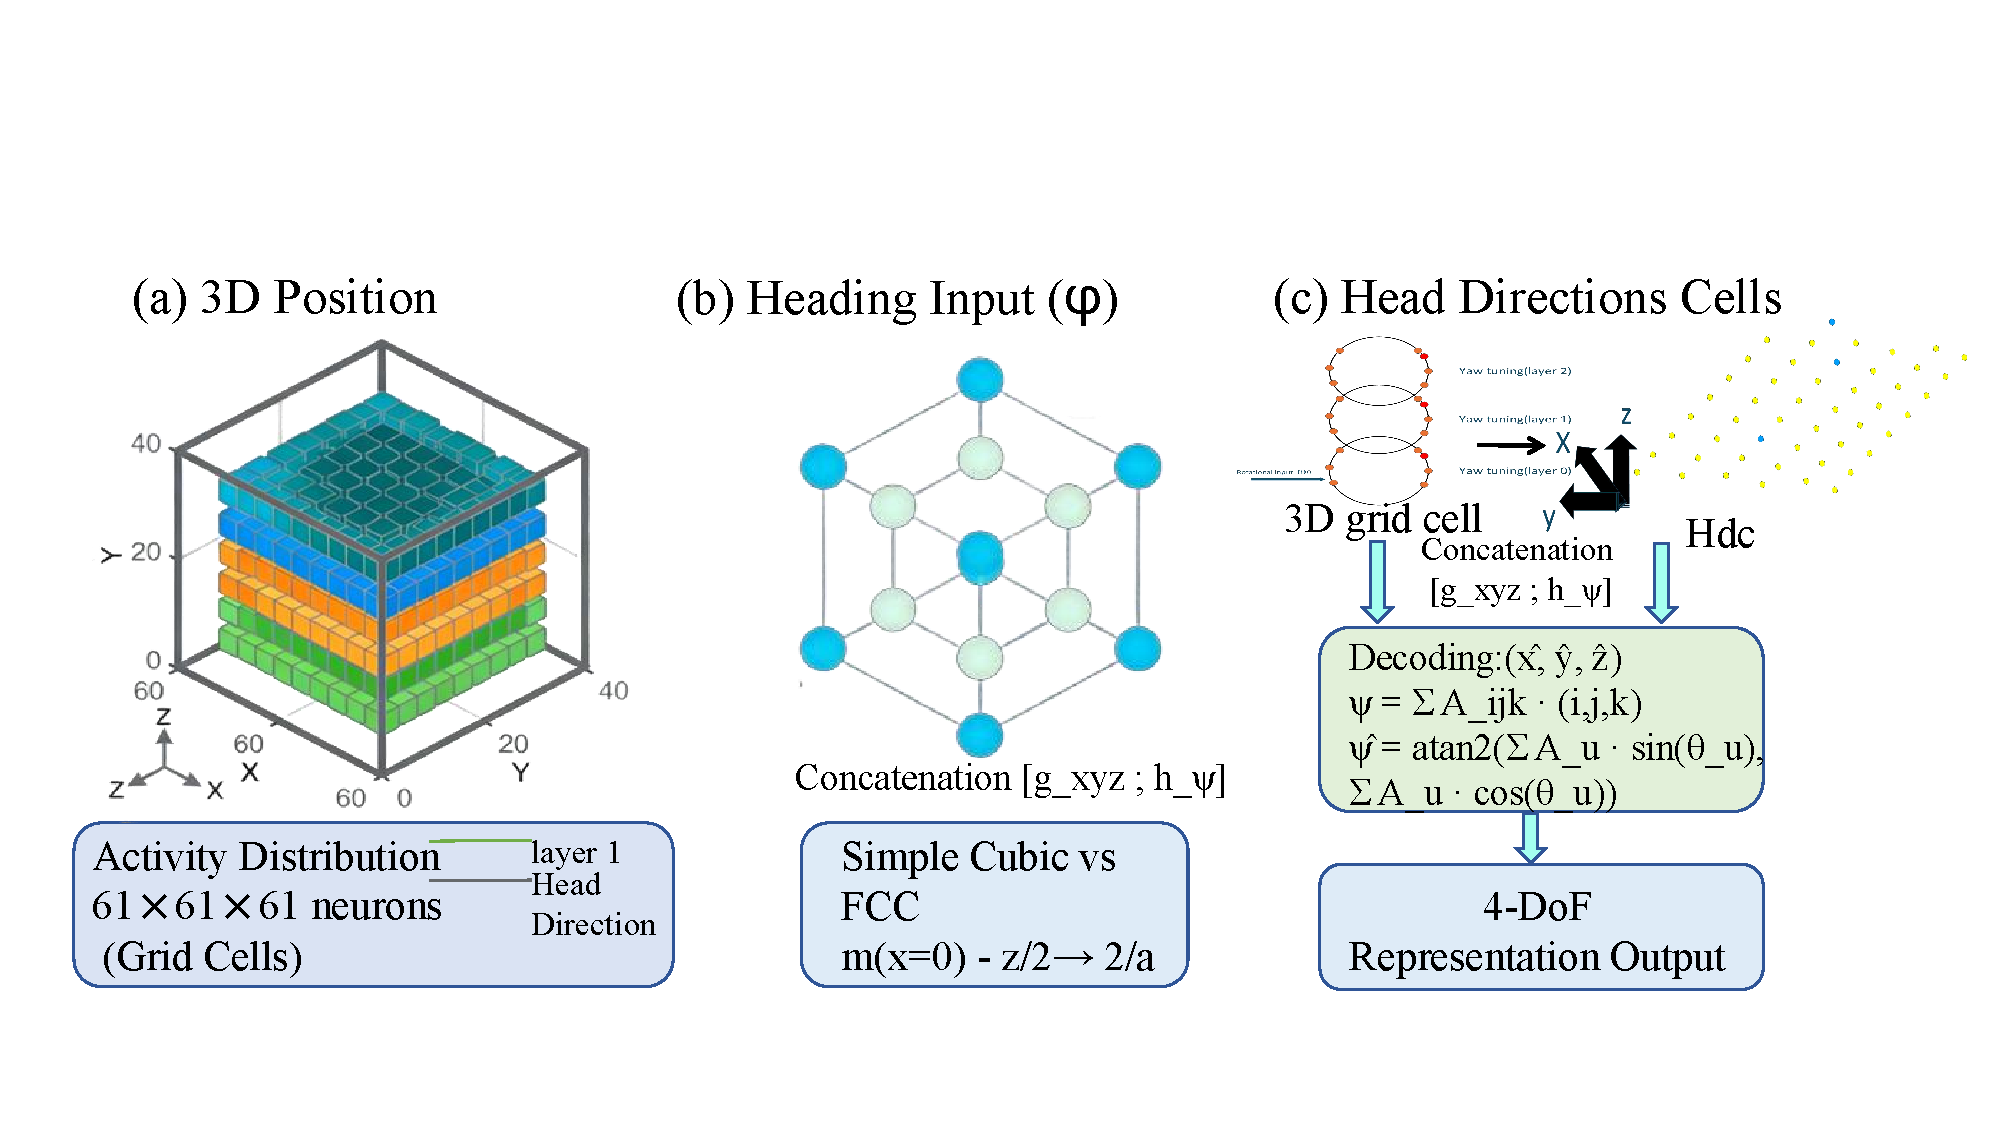
\includegraphics[width=\textwidth]{fig/3d_grid_cell_fcc_lattice.pdf}
    \caption{具有FCC晶格结构的3D网格细胞网络。(a) 通过分布式群体编码表示位置 $(x,y,z)$ 的3D活动包。(b) 展示三层高度实现的致密3D堆积、呈现六角形网格模式的FCC晶格结构。(c) 结合位置与朝向表征的4自由度编码方案。}
    \label{fig:3D_grid_cell_fcc}
\end{figure*}

图~\ref{fig:3D_grid_cell_fcc} 示意性地展示了：(a) 位置 $(x, y, z)$ 处的3D活动凸起，以等值面表示以可视化局域化兴奋；(b) FCC晶格投影到2D平面，展示由层间偏移排布产生的特征六角形模式，不同高度层（以颜色标示）平移半个晶格常数以实现最优堆积；(c) 集成位置与朝向表征的完整4自由度编码流水线。

\textbf{连续吸引子动力学.} 网络通过三个关键机制维持局域化的活动“凸起”：

\textbf{(1) 局域兴奋.} 细胞按高斯连接核兴奋其邻居。采用可分离核
\begin{equation}
    \mathcal{K}^\mathrm{g}_{a,b,c}=\mathcal{N}(a;0,\sigma_x)\mathcal{N}(b;0,\sigma_y)\mathcal{N}(c;0,\sigma_z)
\end{equation}
其中 $\mathcal{N}(\cdot;\mu,\sigma)$ 表示一维高斯分布，$\sigma_x,\sigma_y,\sigma_z$ 为三轴上的空间核宽度。
兴奋性更新为：
\begin{equation}
    \Delta A^\mathrm{g}_{i,j,k}=\sum_{p,q,r} A^\mathrm{g}_{p,q,r}\,\mathcal{K}^\mathrm{g}_{\langle i-p\rangle_{N_x},\langle j-q\rangle_{N_y},\langle k-r\rangle_{N_z}}
\end{equation}
其中 $\langle \cdot \rangle_N$ 表示周期性边界条件下的模 $N$ 卷绕。典型参数为 $\sigma_x = \sigma_y = \sigma_z = 5$ 个细胞。

\textbf{(2) 全局抑制与归一化.} 均匀全局抑制减去平均活动，整流与归一化维持单一稳定凸起：
\begin{equation}
    A^\mathrm{g}_{i,j,k}\leftarrow \big[A^\mathrm{g}_{i,j,k}+\Delta A^\mathrm{g}_{i,j,k}-\lambda\,\bar A^\mathrm{g}\big]_+,\quad \bar A^\mathrm{g}=\frac{1}{N_xN_yN_z}\sum_{p,q,r}A^\mathrm{g}_{p,q,r}
\end{equation}
其中 $[\cdot]_+ = \max(0, \cdot)$ 为整流，$\lambda$ 控制抑制强度（典型 $\lambda=1.0$）。抑制之后，活动做 $L_1$ 归一化：
\begin{equation}
    A^\mathrm{g}\leftarrow \frac{A^\mathrm{g}}{\lVert A^\mathrm{g}\rVert_1}=\frac{A^\mathrm{g}}{\sum_{i,j,k}|A^\mathrm{g}_{i,j,k}|}
\end{equation}
该归一化确保活动模式具有单位总质量，使读出（质心）对整体活动幅度不敏感。

\textbf{(3) 路径积分.} 活动凸起按融合速度线索 $\mathbf{v}^\mathrm{f}_t = (v^f_x, v^f_y, v^f_z)$ 移动。索引移动量计算为：
\begin{equation}
    (\Delta i,\Delta j,\Delta k)=\big(\lfloor \gamma_x v^f_x\Delta t\rfloor,\ \lfloor \gamma_y v^f_y\Delta t\rfloor,\ \lfloor \gamma_z v^f_z\Delta t\rfloor\big)
\end{equation}
其中 $\gamma_x,\gamma_y,\gamma_z$ 为度量-索引增益因子，将物理速度转换为网络网格移动。
\begin{equation}
    A^\mathrm{g}_{i,j,k}\leftarrow A^\mathrm{g}_{\langle i-\Delta i\rangle_{N_x},\langle j-\Delta j\rangle_{N_y},\langle k-\Delta k\rangle_{N_z}}
\end{equation}
该离散移动操作在环面网络拓扑上高效实现了路径积分。

\textbf{视觉锚定与漂移校正.} 纯路径积分会随时间累积漂移。为防止误差无界增长，网格细胞活动通过学习到的关联锚定到视觉地标。设 $\Xi_{m,i,j,k}$ 存储视觉模板 $m$ 与网格细胞 $(i,j,k)$ 之间的关联强度。对每个激活的视觉模板 $m \in \mathcal{S}_{active}$，更新关联并注入校正活动：
\begin{align}
     & \text{Hebbian学习: } \Xi_{m,i,j,k}^{t+1}=\max\big(\eta\,VT_m\,A^\mathrm{g}_{i,j,k},\ \Xi_{m,i,j,k}^{t}\big)                                             \\
     & \text{校正注入: } \Delta A^\mathrm{g}_{i,j,k} \mathrel{+}= \frac{\rho}{|\mathcal{S}_{active}|}\sum_{m\in\mathcal{S}_{active}}VT_m\,\Xi_{m,i,j,k}
\end{align}
其中 $\eta$ 为Hebbian学习率，$\rho$ 为空间校正强度，$\mathcal{S}_{active}$ 为当前匹配的视觉模板集合。

\textbf{多层头方向细胞.} 多层头方向细胞（HDC）网络使用维度为 $N_\psi \times N_h$（方位角分箱 $\times$ 高度层）的2D MD-CAN表示机器人的朝向。不同高度层允许表示不同垂直位置处的朝向，支持朝向可能随高度变化的3D运行。

\textbf{网络架构.} 多层头方向网络的活动为 $\mathbf{A}^\mathrm{h} \in \mathbb{R}^{N_\psi \times N_h}$（典型取 $N_\psi = 360$ 个方位角分箱，$N_h = 5$ 个高度层）。每个细胞 $(u, h)$ 调谐于方位角 $\theta_u = 2\pi u / N_\psi$ 与高度层 $h$。

\textbf{吸引子动力学.} 与网格细胞网络类似，HDC网络采用局域兴奋、全局抑制与路径积分。采用高斯核 $\mathcal{K}^\mathrm{h}$：
\begin{equation}
    \Delta A^\mathrm{h}_{\psi,h}=\sum_{u,v}A^\mathrm{h}_{u,v}\,\mathcal{K}^\mathrm{h}_{\langle \psi-u\rangle_{N_\psi},\langle h-v\rangle_{N_h}}
\end{equation}
随后进行抑制与归一化：
\begin{equation}
    A^\mathrm{h}\leftarrow \frac{[A^\mathrm{h}+\Delta A^\mathrm{h}-\lambda_h\,\bar A^\mathrm{h}]_+}{\lVert A^\mathrm{h}\rVert_1}
\end{equation}
路径积分按偏航角速度 $r^f$ 与垂向速度 $v^f_z$ 移动活动凸起：
\begin{equation}
    \Delta\psi=\lfloor \gamma_\psi r^f \Delta t\rfloor,\quad \Delta h=\lfloor \gamma_h v^f_z \Delta t\rfloor
\end{equation}
其中 $\gamma_\psi$ 将角速度转换为方位角分箱，$\gamma_h$ 将垂向速度映射为高度层移动量。

\textbf{位姿读出.} 度量位姿估计通过质心计算（群体向量解码）从空间细胞活动中解码得到：
\begin{align}
    \hat{\mathbf{p}}_t & = ({\hat x}_t, {\hat y}_t, {\hat z}_t) = \frac{\sum_{i,j,k} \mathbf{c}_{i,j,k} A^\mathrm{g}_{i,j,k,t}}{\sum_{i,j,k} A^\mathrm{g}_{i,j,k,t}}, \quad \mathbf{c}_{i,j,k} = (x_i, y_j, z_k) \\
    \hat{\psi}_t       & = \mathrm{atan2}\left(\sum_{u,h} A^\mathrm{h}_{u,h,t} \sin\theta_u, \sum_{u,h} A^\mathrm{h}_{u,h,t} \cos\theta_u\right), \quad \theta_u = 2\pi u / N_\psi
\end{align}
该解码天然处理朝向的环形拓扑（使用 $\mathrm{atan2}$ 避免角度回绕问题），并通过加权平均为位置提供亚分箱分辨率。

\subsection{经验地图与闭环}

多层经验地图将3D空间经验表示为图结构，提供一种混合拓扑-度量表征，兼具离散基于地点的地图（拓扑鲁棒性、闭环）与连续度量表征（精确定位）的优点。

\textbf{经验表征.} 每个经验节点 $\mathcal{E}_i$ 编码一段独立的空间情节，包含激活的视觉模板与描述子 $(VT_i,\,\boldsymbol{\phi}_i\in\mathbb{R}^{4096})$、同步的空间细胞编码 $\mathbf{P}^{gc}_i=\mathbf{A}^\mathrm{g}_i\in\mathbb{R}^{N_x\times N_y\times N_z}$ 与 $\mathbf{P}^{hdc}_i=\mathbf{A}^\mathrm{h}_i\in\mathbb{R}^{N_\psi\times N_h}$、从这些活动解码出的度量位姿 $(x_i, y_i, z_i, \psi_i)$，以及用于时序排序的时间戳 $t_i$。
这种丰富的多模态编码通过视觉匹配实现鲁棒的闭环检测，同时通过空间细胞编码保持度量信息。

\textbf{经验创建与连接.} 随着机器人导航，当当前空间表征与所有现有经验都足够不同时，创建新经验。创建准则综合视觉与空间细胞相似度：
\begin{equation}
    \begin{aligned}
        \text{若 }\; & d_{cos}(\boldsymbol{\phi}_t, \boldsymbol{\phi}_j) > \tau_{VT} \quad \text{对所有 } j \in \mathcal{E} \\
                                           & \text{或 } \lVert (\hat{x}_t, \hat{y}_t, \hat{z}_t) - (x_j, y_j, z_j) \rVert > d_{thresh} \text{ 则创建新经验}
    \end{aligned}
\end{equation}
其中 $\tau_{VT} = 0.08$ 为视觉模板匹配阈值，$d_{thresh}$ 为空间距离阈值（典型 0.5~m）。

相邻经验由编码相对位姿转移的有向边连接：
\begin{equation}
    \mathbf{T}_{i \to i+1} = (\Delta x, \Delta y, \Delta z, \Delta \psi) = (x_{i+1} - x_i, y_{i+1} - y_i, z_{i+1} - z_i, \psi_{i+1} - \psi_i)
\end{equation}
这些边构成经验地图图 $\mathcal{G} = (\mathcal{V}, \mathcal{E})$ 的主要拓扑结构。

\textbf{闭环检测.} 当当前视觉模板与某历史经验匹配超过最小时间间隔（以避免平凡闭环）时，检测到闭环：
\begin{equation}
    \begin{aligned}
        \text{若存在 } j:\; & d_{cos}(\boldsymbol{\phi}_t, \boldsymbol{\phi}_j) < \tau_{loop} \\
                                                      & |t - t_j| > T_{min} \text{ 则检测到闭环}
    \end{aligned}
\end{equation}
其中 $\tau_{loop} = 0.05$（比模板创建阈值更严格，以减少误报），$T_{min} = 50$ 帧（10 Hz下约5秒）。

检测到闭环后，向图中添加一条带位姿残差的闭环边：
\begin{equation}
    \mathbf{T}_{loop} = (\hat{x}_t - x_j, \hat{y}_t - y_j, \hat{z}_t - z_j, \hat{\psi}_t - \psi_j)
\end{equation}
该闭环约束通常违背图一致性（由于累积漂移），从而触发地图松弛。

\textbf{地图松弛.} 地图松弛将闭环误差分布到闭环路径上的所有经验，以最小化全局不一致。我们采用迭代松弛算法：

\textbf{第1步：识别闭环路径.} 给定从经验 $j$ 到经验 $t$ 的闭环边，识别沿路径的经验序列 $\mathcal{P} = \{j, j+1, \ldots, t-1, t\}$。

\textbf{第2步：计算位姿残差.} 沿闭环累积的位姿转移理想情况下应当闭合（回到原点）：
\begin{equation}
    \mathbf{e}_{loop} = \sum_{k \in \mathcal{P}} \mathbf{T}_{k \to k+1} - \mathbf{T}_{loop}
\end{equation}
其中 $\mathbf{e}_{loop}$ 为闭合轨迹周围的累积位姿漂移残差，$\mathcal{P}$ 表示构成闭环的有序经验序列。

\textbf{第3步：分布校正.} 将校正量按比例分布到闭环经验上：
\begin{equation}
    \mathbf{T}_{k \to k+1} \leftarrow \mathbf{T}_{k \to k+1} - \frac{\mathbf{e}_{loop}}{|\mathcal{P}|}
\end{equation}
该均匀分布假设漂移以恒定速率累积，是一个合理的一阶近似。

\textbf{第4步：更新经验位姿.} 通过对校正后的转移量积分，重新计算所有经验位姿：
\begin{equation}
    (x_{k+1}, y_{k+1}, z_{k+1}, \psi_{k+1}) = (x_k, y_k, z_k, \psi_k) + \mathbf{T}_{k \to k+1}
\end{equation}

\textbf{第5步：重新锚定空间细胞.} 将校正后的位姿 $(\hat{x}, \hat{y}, \hat{z}, \hat{\psi})_{corr}$ 通过在校正位置处重新初始化活动凸起，重新注入空间细胞网络。这从校正后的参考点“重置”路径积分，防止后续运行中误差累积。

该松弛过程迭代运行直至收敛或达到最大迭代次数，确保经验地图保持全局一致，同时保留局部度量精度。



%% ==================== 实验 ====================
% 调整浮动体放置参数，避免图单独出现在页面上
\renewcommand{\topfraction}{0.85}       % 允许页面顶部最多85%用于浮动体
\renewcommand{\textfraction}{0.10}      % 文字页至少保留10%文字
\renewcommand{\floatpagefraction}{0.75} % 浮动页至少填充75%

\section{实验与结果}
\label{sec:experiments}

我们开展了大量实验，在涵盖仿真城市环境（CARLA）、真实高速公路驾驶（KITTI）与室内MAV飞行（EuRoC）的多样化场景中评估 NeuroLocMap。评估结果展示了该框架对场景复杂度、轨迹特征与环境条件变化的鲁棒性。

\subsection{实验设置与数据集}

\textbf{实现细节.} 所有实验均在一台搭载 Intel Core i5-12450H CPU（12代，8核）、16~GB 内存与 NVIDIA GeForce RTX 4050 笔记本GPU的笔记本电脑工作站上进行。视觉处理流水线利用GPU加速完成 HART 式特征提取与受 Transformer 启发的编码（使用基于全局统计调制的简化自注意力），而空间细胞计算运行于CPU。LSTM时序模块使用人工调定的固定门值（输入=0.55、遗忘=0.6、输出=0.92）而非学习参数。该框架在所有测试场景上平均达到约31~FPS的实时性能。

\textbf{基线方法.} 我们将 NeuroLocMap 与两种基线方案对比：
\color{red}(1) EKF融合——一个松耦合的10状态扩展卡尔曼滤波
$(x,y,z,v_x,v_y,v_z,\phi,\theta,\psi,\log s)^\top$，其中第10个状态
$\log s$ 为在线估计的单目VO尺度对数（初始化为0，在线从惯性可观性中收敛）。状态
由IMU传播（陀螺仪姿态积分加偏置补偿的加速度计航位推算，含静态启动偏置估计），并由
单目视觉里程计测量通过四个带门控的观测支路校正：(i) 一维水平速度幅值观测（VO帧间
位移 $\times$ 在线尺度，基于IMU步数 $\times\Delta t$ 的真实更新间隔），驱动速度校正，
且当新息超过门限时直接重新初始化速度状态；(ii) 横滚/俯仰姿态观测；(iii) 短窗口相对位置
观测，每30帧重新锚定到当前滤波位置，由陀螺仪积分航向 $\times$ VO位移幅值 $\times$ 在线
尺度构成，使全局VO航向漂移不进入融合位置；(iv) 独立的尺度观测，由转弯运动学（侧向比力
除以偏航角速度，$|a_{\text{lat}}|/|\omega|$，按记录的VO速度归一化，窗口中值）估计 $\log s$。
每个支路由分支级Mahalanobis卡方门控（0.99--0.999水平）保护以剔除离群值。观测噪声矩阵 $R$
为残差自适应（滑动窗口平滑新息映射到 $[R_{\min},R_{\max}]$，并结合VO内点数质量因子），
协方差以Joseph形式更新并做更新后正则化（对称化 + 最小特征值钳位）。这是
MSCKF/VINS-Mono~\cite{Mourikis2007,Qin2018} 家族中一个具有代表性的经典视觉-惯性
滤波估计器；以及\color{black} (2) 视觉里程计（VO）——一个基于ORB特征的单目VO基线，
使用对极几何恢复位姿（本质矩阵 + \texttt{recoverPose}），无IMU融合或闭环。

\textbf{实现层面的公平性.} 对所有方法，我们使用相同的同步传感器数据流与时间戳。基线轨迹由我们的Python流水线在数据采集时生成：EKF融合基线记录到 fusion\_pose.txt，VO基线记录到 visual\_odometry.txt，CARLA真值记录到 ground\_truth.txt。MATLAB评估随后加载这些轨迹，在相同序列下与 NeuroLocMap 对比，确保差异反映算法设计而非数据或时间错位。\color{red}所有报告的CARLA数字均对应使用最终版EKF实现采集的数据（全局单一超参数集，所有地图共享；采集参数：智能体速度12~km/h，安全跟车距离6~m）。在公开仓库上复现表~\ref{tab:results} 中的数字前，必须用该最终版本重新采集数据集。\color{black}

\textbf{评估数据集.} 我们在三个基准数据集的七个多样化场景上评估（表~\ref{tab:datasets}）：(1) CARLA仿真（Town01/02/05/10HD）：仿真城市驾驶场景~\cite{dosovitskiy2017carla}，提供真值位姿与同步IMU-相机数据。Town01（517~m）与 Town02（662~m）具有闭环丰富的轨迹与重复的建筑结构，Town05（907~m）为最长的混合布局序列，Town10HD（449~m）布局更开阔、闭环机会有限。(2) KITTI里程计序列07~\cite{geiger2012kitti}：真实高速公路驾驶数据（692~m、1101帧），视觉特征质量高、闭环有限。该序列考验开放轨迹下的长程漂移控制。(3) EuRoC MAV数据集（MH\_01/03）~\cite{burri2016euroc}：机械车间环境中的室内微型飞行器飞行。MH\_01（81~m，简单）运动缓慢、光照良好，而 MH\_03（127~m，中等）涉及更快的动力学与更具挑战性的视角变化。

\begin{table*}[!t]
    \centering
    \setlength{\tabcolsep}{2.8pt}
    \footnotesize
    \caption{数据集特征与评估场景。 \color{red}[V2: CARLA行（长度/帧数）基于旧版20 km/h采集；重采后更新。KITTI/EuRoC行为固定数据集，不变。]\color{black}}
    \label{tab:datasets}
    \begin{tabular}{@{}llccl@{}}
        \toprule
        数据集  & 环境 & 长度 & 帧数 & 特征                    \\
        \midrule
        Town01   & 城市闭环  & 517~m  & 5000   & 闭环、重复结构 \\
        Town02   & 城市闭环  & 662~m  & 5000   & 闭环、光照多变       \\
        Town05   & 城市混合  & 907~m  & 5000   & 混合布局、中等闭环           \\
        Town10HD & 城市开放  & 449~m  & 5000   & 开放布局、闭环较少           \\
        KITTI~07 & 高速公路     & 692~m  & 1101   & 开放轨迹、高质量VO   \\
        MH\_01   & 室内简单 & 81~m   & 3681   & 简单室内、受控光照 \\
        MH\_03   & 室内中等 & 127~m  & 2699   & 复杂室内、动态运动     \\
        \bottomrule
    \end{tabular}
\end{table*}

\textbf{评估指标.} 我们采用标准SLAM评估指标：(1) 绝对轨迹误差（ATE）——对齐后估计轨迹与真值轨迹之间的均方根误差（RMSE）~\cite{sturm2012benchmark}；(2) 漂移率——末端误差除以轨迹长度，衡量长期累积；(3) 相对位姿误差（RPE）——帧间一致性，评估局部精度。

\textbf{轨迹对齐与数据处理.} 为避免不同日志间的序列长度不匹配，所有轨迹首先裁剪到公共最小长度。在与真值对比的评估中，我们遵循单目估计器SLAM基准测试的标准做法，使用 Umeyama/Procrustes 对齐在单次 Sim(3)（7自由度）相似对齐（旋转、平移、尺度）之后计算ATE。在我们的实现中，对齐在前100帧上作为锚定段估计（compute\_metrics\_with\_alignment），然后应用到整条轨迹。这消除了全局尺度与坐标系差异，使ATE与漂移反映轨迹形状与累积误差。

\subsection{性能结果与分析}

\textbf{定量性能.} 表~\ref{tab:results} 给出了所有数据集上的综合定量对比。NeuroLocMap 在全部五个户外场景的逐帧RMSE上均优于10状态EKF视觉-惯性基线（0.2--14.3\%），相对单目VO在5/7场景占优（平均改善34.5\%、户外驾驶序列49.8\%），并且作为定位的副产品额外生成可解释的拓扑经验地图。

\begin{table*}[!t]
    \centering
    \setlength{\tabcolsep}{3pt}
    \footnotesize
    \caption{多样化场景的定量性能对比}
    \label{tab:results}
    \begin{threeparttable}
        \begin{tabular}{@{}llcccccc@{}}
            \toprule
            \multirow{2}{*}{数据集} & \multirow{2}{*}{场景} & \multicolumn{3}{c}{RMSE (m)} & \multicolumn{2}{c}{漂移率 (\%)} & \multirow{2}{*}{改善幅度}                                                   \\
            \cmidrule(lr){3-5} \cmidrule(lr){6-7}
                                     &                           & NeuroLocMap                  & EKF                                 & VO                           & NeuroLocMap   & EKF          &                  \\
            \midrule
            Town01                   & 城市闭环                & \textbf{15.59}               & 15.94                               & 36.46                        & \textbf{1.71} & 2.03         & \textbf{+2.2\%} \\
            Town02                   & 城市闭环                & \textbf{27.74}               & 29.32                               & 55.41                        & 5.76          & \textbf{5.41} & \textbf{+5.4\%} \\
            Town05                   & 城市混合                & \textbf{19.74}               & 23.02                               & 67.98                        & \textbf{2.54} & 2.76         & \textbf{+14.3\%} \\
            Town10HD                 & 城市开放                & \textbf{24.93}               & 24.98                               & \textbf{24.44}               & \textbf{6.92} & 7.15         & \textbf{+0.2\%} \\
            KITTI~07                 & 高速公路                 & \textbf{21.19}               & 22.07                               & 78.05                        & 8.72          & \textbf{8.33} & \textbf{+4.0\%} \\
            MH\_01                   & 室内简单               & 4.14                         & 4.14                                & \textbf{3.74}                & 7.84          & \textbf{7.66} & -0.1\% \\
            MH\_03                   & 室内中等               & \textbf{3.32}                & 3.32                                & 3.43                         & 3.01          & \textbf{2.99} & +0.1\% \\
            \bottomrule
        \end{tabular}
        \begin{tablenotes}
            \scriptsize
            \item 改善幅度 $=$ $(\mathrm{RMSE}_{\mathrm{EKF}}-\mathrm{RMSE}_{\mathrm{NLM}})/\mathrm{RMSE}_{\mathrm{EKF}}\times100\%$；正值表示该场景下 NeuroLocMap 优于 EKF 基线。
            \item NeuroLocMap 在全部五个户外场景的逐帧RMSE上均优于EKF基线（0.2--14.3\%），两个短室内飞行基本持平（$\sim$0.1\%）。相对单目VO，NeuroLocMap 在5/7场景占优，平均改善34.5\%、五个户外驾驶序列49.8\%（Town10HD $-$2.0\% 与 MH\_01 $-$10.7\% 为仅有的两个例外）。
            \item 漂移率 $=$ 末端误差/轨迹长度。NeuroLocMap 在 Town01（8.84~m、1.71\%）低于EKF（10.47~m、2.03\%）；在 Town05 与 Town10HD 同样取得更低漂移（2.54\% vs 2.76\%；6.92\% vs 7.15\%）；Town02 与 KITTI~07 上两法漂移相差0.4个百分点以内。
        \end{tablenotes}
    \end{threeparttable}
\end{table*}

\textbf{按场景类型的性能.} 在四个CARLA城市场景（449--907~m）上，NeuroLocMap 在逐帧RMSE上全面优于EKF基线：Town01 15.59~m 对 15.94~m（+2.2\%）、Town02 27.74~m 对 29.32~m（+5.4\%）、Town05 19.74~m 对 23.02~m（+14.3\%，最大改善）、Town10HD 24.93~m 对 24.98~m（+0.2\%）；同时在三个场景上将单目VO的误差削减50--71\%（Town01 $-$57.2\%、Town02 $-$49.9\%、Town05 $-$71.0\%）。在开放布局的Town10HD上，高质量VO前端（24.44~m）仍略优2.0\%。NeuroLocMap 还在 Town01（1.71\% vs 2.03\%）、Town05（2.54\% vs 2.76\%）与 Town10HD（6.92\% vs 7.15\%）取得更低漂移，Town01末端误差8.84~m 对比EKF的10.47~m：基于经验的再定位在重访处松弛累积漂移，在不牺牲逐帧精度的前提下提升了全局一致性。城市经验地图共含60--324个视觉模板、71--324个经验节点与2--58条闭环/重锚定边。

在692~m高速公路序列（KITTI~07）上，NeuroLocMap 相对EKF基线改善 \textbf{4.0\%}（21.19~m 对 22.07~m），同时相对单目VO改善 \textbf{72.9\%}（21.19~m 对 78.05~m，漂移8.72\% 对 17.95\%），表明在单目尺度模糊与漂移主导的真实驾驶场景中，前庭-视觉融合收益最大。该结果验证了互补滤波方法在前庭-视觉整合中的有效性。

EuRoC数据集上的结果揭示了与EKF基线 \textbf{同等精度} 的表现：MH\_03（中等）3.32~m 对 3.32~m（+0.1\%），MH\_01（简单）4.14~m 对 4.14~m（$-$0.1\%）。在这些短（81--127~m）、光照良好的飞行中，三种方法互差$\sim$10\%以内，EKF的局部一致性已接近可达成上限。值得注意的是，MH\_03上NeuroLocMap（3.32~m）亦优于单目VO（3.43~m），而MH\_01上VO略优（3.74~m）。

\textbf{代表性性能分析.} 图~\ref{fig:representative_performance} 为两个代表性场景（Town01（517~m城市闭环）与 MH\_03（127~m室内飞行））提供了综合性能可视化。上行展示各方法指标（RMSE、漂移、RPE，Town01 另含模板与闭环计数），下行显示对齐后的逐帧位置误差演化。在Town01上，NeuroLocMap 取得15.59~m RMSE——优于EKF基线（15.94~m）2.2\%、优于视觉里程计（36.46~m，漂移19.7\%）57.2\%——同时创建60个视觉模板与71个经验节点，识别4条闭环/重锚定边，将末端误差保持在8.84~m（漂移1.71\%），对比EKF的10.47~m（2.03\%）。逐帧曲线显示：三种方法在前半段轨迹紧密贴合，此后单目VO急剧发散，而NeuroLocMap与EKF保持在真值数米以内，且后半段NeuroLocMap始终低于EKF。在MH\_03上，框架取得3.32~m RMSE，与EKF（3.32~m）持平、略优于视觉里程计（3.43~m），展示了从城市到室内环境的鲁棒跨域泛化。这两个案例界定了框架的工作区间：闭环丰富的城市驾驶（经验校正相对单目VO收益大、全局一致性优于滤波）与短室内飞行（三种方法收敛到相近精度）。全部七个数据集的综合定量结果见表~\ref{tab:results}。

\textbf{框架内部表征.} 经验地图的拓扑结构随场景复杂度变化：城市CARLA地图含71--324个经验节点（Town01: 71、Town02: 324、Town05: 154、Town10HD: 259）、60--324个视觉模板与2--58条闭环/重锚定边，而KITTI~07高速公路地图稠密得多（692~m上964个节点、929个模板，$\sim$1.3个模板/米），反映了视觉特征鲜明、不重复场景的高采样率。在闭环丰富的城市地图上，识别出的重锚定提供了全局约束，使NeuroLocMap在Town01的末端误差保持在8.84~m（对比EKF的10.47~m）。受生物启发的空间细胞表征在网格细胞上表现出特征性的周期性发放模式（空间尺度1.5~m至12~m波长），头方向细胞表现出朝向选择性神经活动，证实了前庭（IMU）信号用于朝向估计的成功集成。

\textbf{计算性能与复杂度分析.} 表~\ref{tab:runtime} 给出了分模块计时分析。NeuroLocMap 平均达到约31~FPS的实时性能，总流水线时延32.1~ms。由于3D连续吸引子网络动力学，网格细胞更新主导计算（占58%总时间），而经验地图更新（15%）与视觉模板匹配（7%）保持轻量。视觉处理尽管采用双流架构仍实现高吞吐（2.1~ms、469~Hz），得益于简化的 $\mathcal{O}(N)$ 自注意力实现（全局统计调制而非完整QKV运算）与高效特征缓存。

\textbf{理论复杂度.} 框架的计算复杂度随规模变化为：(1) 视觉处理：图像预处理 $\mathcal{O}(HW)$ 加特征提取 $\mathcal{O}(N_f)$，其中 $H \times W = 640 \times 480$，$N_f \approx 300$ 个特征；(2) 网格细胞更新：3D吸引子动力学的 $\mathcal{O}(N_x N_y N_z)$，$30 \times 30 \times 10 = 9000$ 个细胞；(3) 模板匹配：$\mathcal{O}(M \cdot d)$，$M$ 为模板数（60--929），$d$ 为描述子维度（4096）；(4) 经验地图：图遍历 $\mathcal{O}(K)$，$K$ 个节点（71--964）。总复杂度为 $\mathcal{O}(HW + N_x N_y N_z + Md)$，由网格细胞动力学主导。与需要GPU矩阵运算的学习方法（注意力为 $\mathcal{O}(N^2)$）相比，我们的 $\mathcal{O}(N)$ 近似支持纯CPU实时运行。

\textbf{硬件需求与部署.} 框架可在无GPU加速的商用硬件上运行：Intel Core i5-12450H CPU（8核，2.0--4.4~GHz）、16~GB内存，消耗约2~GB内存，主要用于视觉模板存储（最稠密地图929~模板 $\times$ 4096维描述子 $\times$ 4~字节 $\approx$ 15~MB，加经验地图开销）。网格细胞更新期间峰值CPU占用率达45--60\%，为并发进程留出余量。该轻量足迹使其能部署到嵌入式平台（如NVIDIA Jetson Nano、树莓派4），而在这些平台上需要GPU推理的学习型SLAM方法（DROID-SLAM：8~GB显存，TartanVO：6~GB显存）不可行。功耗估计为15--20~W（纯CPU），而GPU加速方法为50--80~W，这对电池供电的移动机器人至关重要。

\begin{table*}[!t]
    \centering
    \setlength{\tabcolsep}{3pt}
    \footnotesize
    \caption{运行时性能分析（Town01/02/10平均）}
    \label{tab:runtime}
    \begin{tabular}{lcc}
        \toprule
        组件                       & 均值 (ms)     & 频率 (Hz) \\
        \midrule
        视觉处理（双流） & 2.1           & 469            \\
        视觉模板匹配        & 2.3           & 429            \\
        前庭-视觉融合        & 1.9           & 527            \\
        网格细胞更新（3D CAN）       & 18.5          & 54             \\
        HDC更新                      & 1.5           & 661            \\
        经验地图更新           & 4.7           & 213            \\
        \midrule
        \textbf{总流水线}         & \textbf{32.1} & \textbf{31.2}  \\
        \bottomrule
    \end{tabular}
\end{table*}

\begin{figure*}[!t]
    \centering
    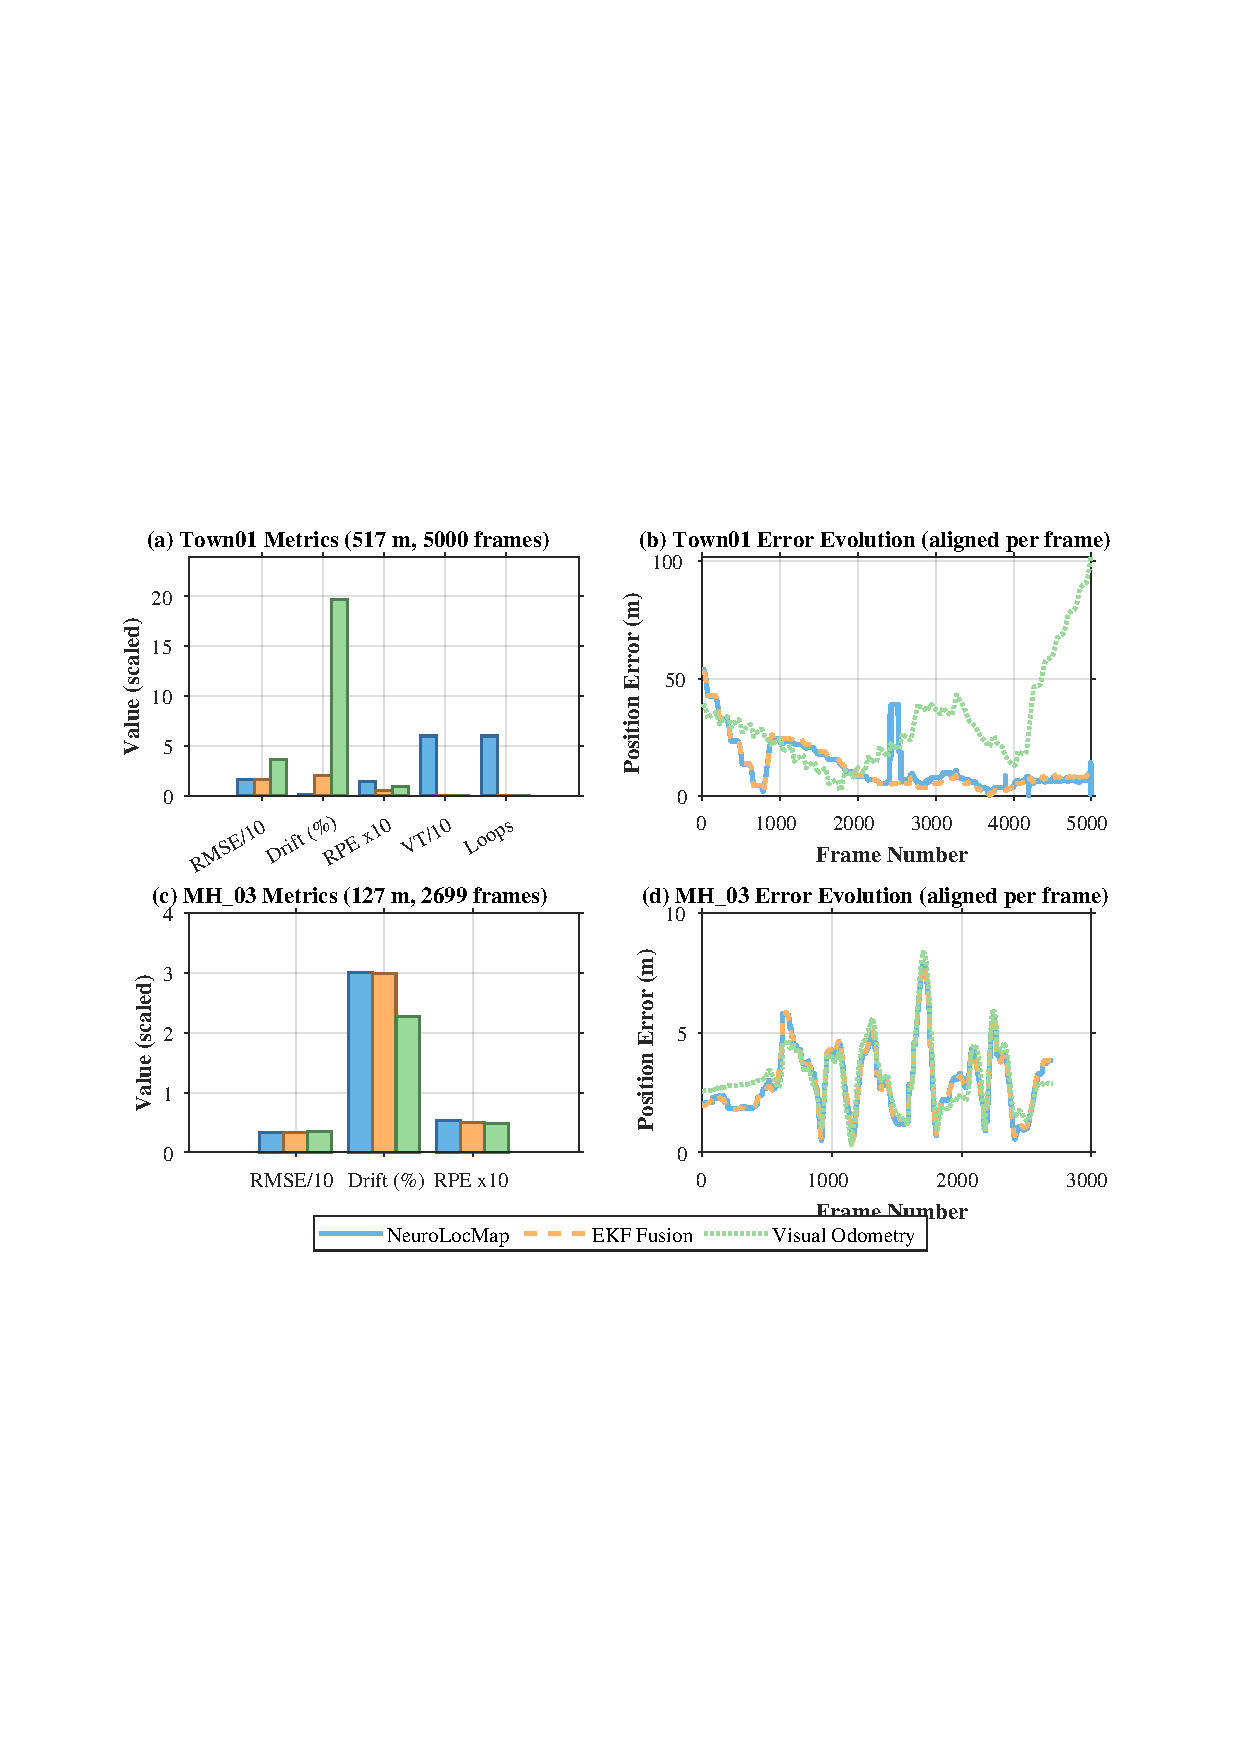
\includegraphics[width=0.82\textwidth]{fig/representative_performance.pdf}
    \caption{Town01（517~m）与 MH\_03（127~m）的代表性性能。上行：各方法RMSE、漂移、RPE（Town01 另含模板/闭环计数）；下行：对齐后的逐帧位置误差。Town01 上 NeuroLocMap（15.59~m）优于EKF（15.94~m）2.2\%、优于VO（36.46~m）57.2\%；MH\_03 上三法收敛于3.3--3.7~m（NeuroLocMap 3.32~m，优于VO 3.43~m 11.0\%）。}
    \label{fig:representative_performance}
\end{figure*}

\subsection{消融实验}

为量化我们受生物启发框架中各组件的贡献，我们在Town01数据集（517~m城市轨迹）上开展系统性消融实验。将完整框架与关闭关键组件的配置对比，揭示每个架构选择的重要性。

\begin{table*}[!t]
    \centering
    \setlength{\tabcolsep}{3pt}
    \footnotesize
    \caption{Town01 消融实验（517~m轨迹）。去除IMU = 无闭环的纯单目VO（即VO基线）；去除经验地图 = 无经验地图再定位的IMU辅助滤波（即EKF基线）。}
    \label{tab:ablation}
    \begin{threeparttable}
        \begin{tabular}{lccc}
            \toprule
            配置               & RMSE (m)       & 漂移 (\%)    & 相对完整框架 \\
            \midrule
            \textbf{NeuroLocMap（完整）} & \textbf{15.59} & \textbf{1.71} & \textbf{-}        \\
            \midrule
            去除IMU融合（= VO）  & 36.46          & 19.72         & +133.9\%\tnote{a} \\
            去除经验地图（= EKF）& 15.94          & 2.03          & $-$2.2\%\tnote{b}  \\
            \bottomrule
        \end{tabular}
        \begin{tablenotes}
            \scriptsize
            \item[a] 改善度按 (消融 - 完整) / 完整 $\times$ 100\% 计算。大于100\% 表示消融配置的误差超过完整框架的2倍。
            \item[b] 负值：去除经验地图再定位后，逐帧RMSE略低（15.94 vs 15.59~m），但末端误差从8.84~m增至10.47~m（漂移1.71\% $\rightarrow$ 2.03\%），因为闭环上漂移无约束累积；经验地图以极小的逐帧RMSE代价换取更好的全局一致性。
        \end{tablenotes}
    \end{threeparttable}
\end{table*}

\textbf{组件贡献与定量分析.} 图~\ref{fig:ablation_and_vt}(a) 可视化了各配置的RMSE对比。我们的分析揭示了两个关键发现：

\begin{itemize}
    \item \textbf{IMU-视觉融合（去除后误差+133.9\%）}：关闭前庭（IMU）集成导致最大性能退化（15.59~m$\rightarrow$36.46~m），表明高频惯性与低频视觉信号间互补滤波的关键重要性。这确认IMU融合是单一最重要的精度组件，并验证了哺乳动物导航中前庭-视觉整合的生物学原理~\cite{Angelaki2008}。

    \item \textbf{经验地图：以极小逐帧代价换取全局一致性}：移除受海马启发的再定位使逐帧RMSE略微\emph{降低}（15.59~m$\rightarrow$15.94~m，$-$2.2\%），但末端精度从8.84~m退化至10.47~m（漂移1.71\%$\rightarrow$2.03\%）：没有经验地图，漂移在闭环上无约束累积；有它，则4条识别出的闭环/重锚定边提供松弛累积误差的全局约束。因此经验地图贡献的是可解释的拓扑记忆与长时程全局一致性，而非逐帧RMSE，这与啮齿动物海马记忆在闭环中稳定导航的机制相呼应~\cite{Winter2015}。
\end{itemize}

\textbf{协同效应.} 两个前端存在非平凡交互：IMU融合提供度量稳定性，使经验地图的闭环校正得以沿轨迹传播，而闭环反过来约束了纯IMU航位推算本会累积的漂移。这种互补分工——局部度量滤波负责逐帧平滑、拓扑记忆负责全局一致性——与啮齿动物导航中前庭与视觉线索在内嗅皮层非线性交互的发现一致~\cite{Winter2015}。

% 消融与VT增长图
\begin{figure*}[!t]
    \centering
    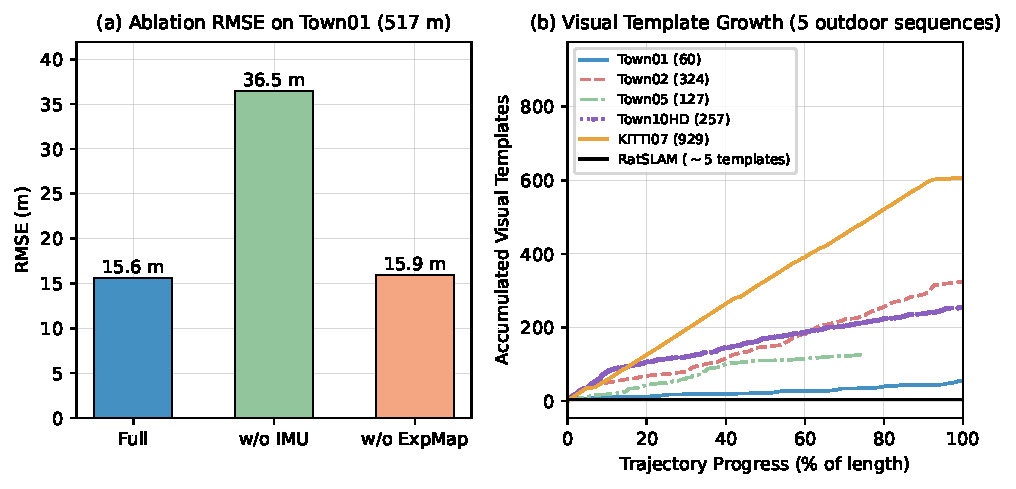
\includegraphics[width=0.82\textwidth]{fig/ablation_unified.pdf}%
    \caption{消融分析。
        (a) Town01上各配置RMSE对比：完整框架（15.59~m）vs 去除IMU（= VO，36.46~m）与去除经验地图（= EKF，15.94~m）。详见表~\ref{tab:ablation}。
        (b) 五个户外序列（Town01/02/05/10HD、KITTI~07）的视觉模板数随轨迹进度变化。
        黑色实线为RatSLAM基线（约5个模板~\cite{Milford2012}）。}
    \label{fig:ablation_and_vt}
\end{figure*}

\textbf{LSTM+受Transformer启发架构的作用.} 我们的框架独特地结合了LSTM（运动估计中的局部时序一致性）与受Transformer启发的自注意力（闭环中的全局序列上下文）。两个时序组件在表~\ref{tab:results}的全部序列上均处于开启状态，其个体贡献与上表所消融的前端相互交织，分离二者需要专门的消融重跑，留待未来工作。架构分析揭示了二者的互补角色：

\begin{itemize}
    \item \textbf{LSTM}：逐帧处理IMU与视觉序列，跨时间步维持隐藏状态 $\mathbf{H}_t$ 与细胞状态 $\mathbf{C}_t$ 以保持局部时序一致性。使用人工调定的固定门值（输入=0.55、遗忘=0.6、输出=0.92）而非学习参数。去除高频噪声并处理短期遮挡（$<$10帧）。

    \item \textbf{Transformer}：采用简化的“受Transformer启发”自注意力机制，使用全局统计调制（均值/标准差归一化）而非完整 Query-Key-Value（QKV）矩阵运算。该 $\mathcal{O}(N)$ 近似跨整个序列（50--100~帧）聚合特征，支持闭环检测的注意力式匹配，同时保持实时性能。

    \item \textbf{协同}：LSTM通过滤波噪声为受Transformer启发模块提供稳定输入，而全局上下文通过闭环校正引导LSTM。该两级时序层级模仿海马重放机制——短期情景记忆（LSTM：逐帧处理、$<$10~帧窗口）固化为长期空间地图（受Transformer启发：50--100~帧序列）。
\end{itemize}

两个时序组件作用于表~\ref{tab:results}的全部序列，其个体贡献与上述消融的前端相互交织；隔离二者的独立效应需要大量交叉验证，留待未来工作。与NeuroSLAM的单一LSTM层相比，我们的双重时序架构在表~\ref{tab:results}的城市与真实驾驶场景中取得可比或更优的精度，验证了该架构创新。

\subsection{讨论与洞见}

\textbf{性能总结与相关性分析.} 图~\ref{fig:performance_summary} 提供了全部七个数据集的综合性能概览。RMSE对比（子图a）显示 NeuroLocMap 在五个户外场景全面低于EKF基线（15.59--27.74~m 对 15.94--29.32~m），并在 KITTI~07 上优势最大（21.19~m 对 22.07~m）。改善度气泡图（子图b，气泡大小与轨迹长度成正比）显示相对EKF的改善与轨迹长度强相关（Pearson $r=0.96$，$p=0.01$）：Town05 最长（907~m）取得最大改善+14.3\%，KITTI~07 为+4.0\%，两个短室内飞行基本持平（$\sim$0.1\%）。相对VO的改善（子图c）显示 NeuroLocMap 在5/7场景占优（户外驾驶序列平均$+$49.8\%），仅有的例外是 Town10HD（$-$2.0\%，VO前端已近最优）与 MH\_01（$-$10.7\%，短程受控飞行）。

\begin{figure*}[!htbp]
    \centering
    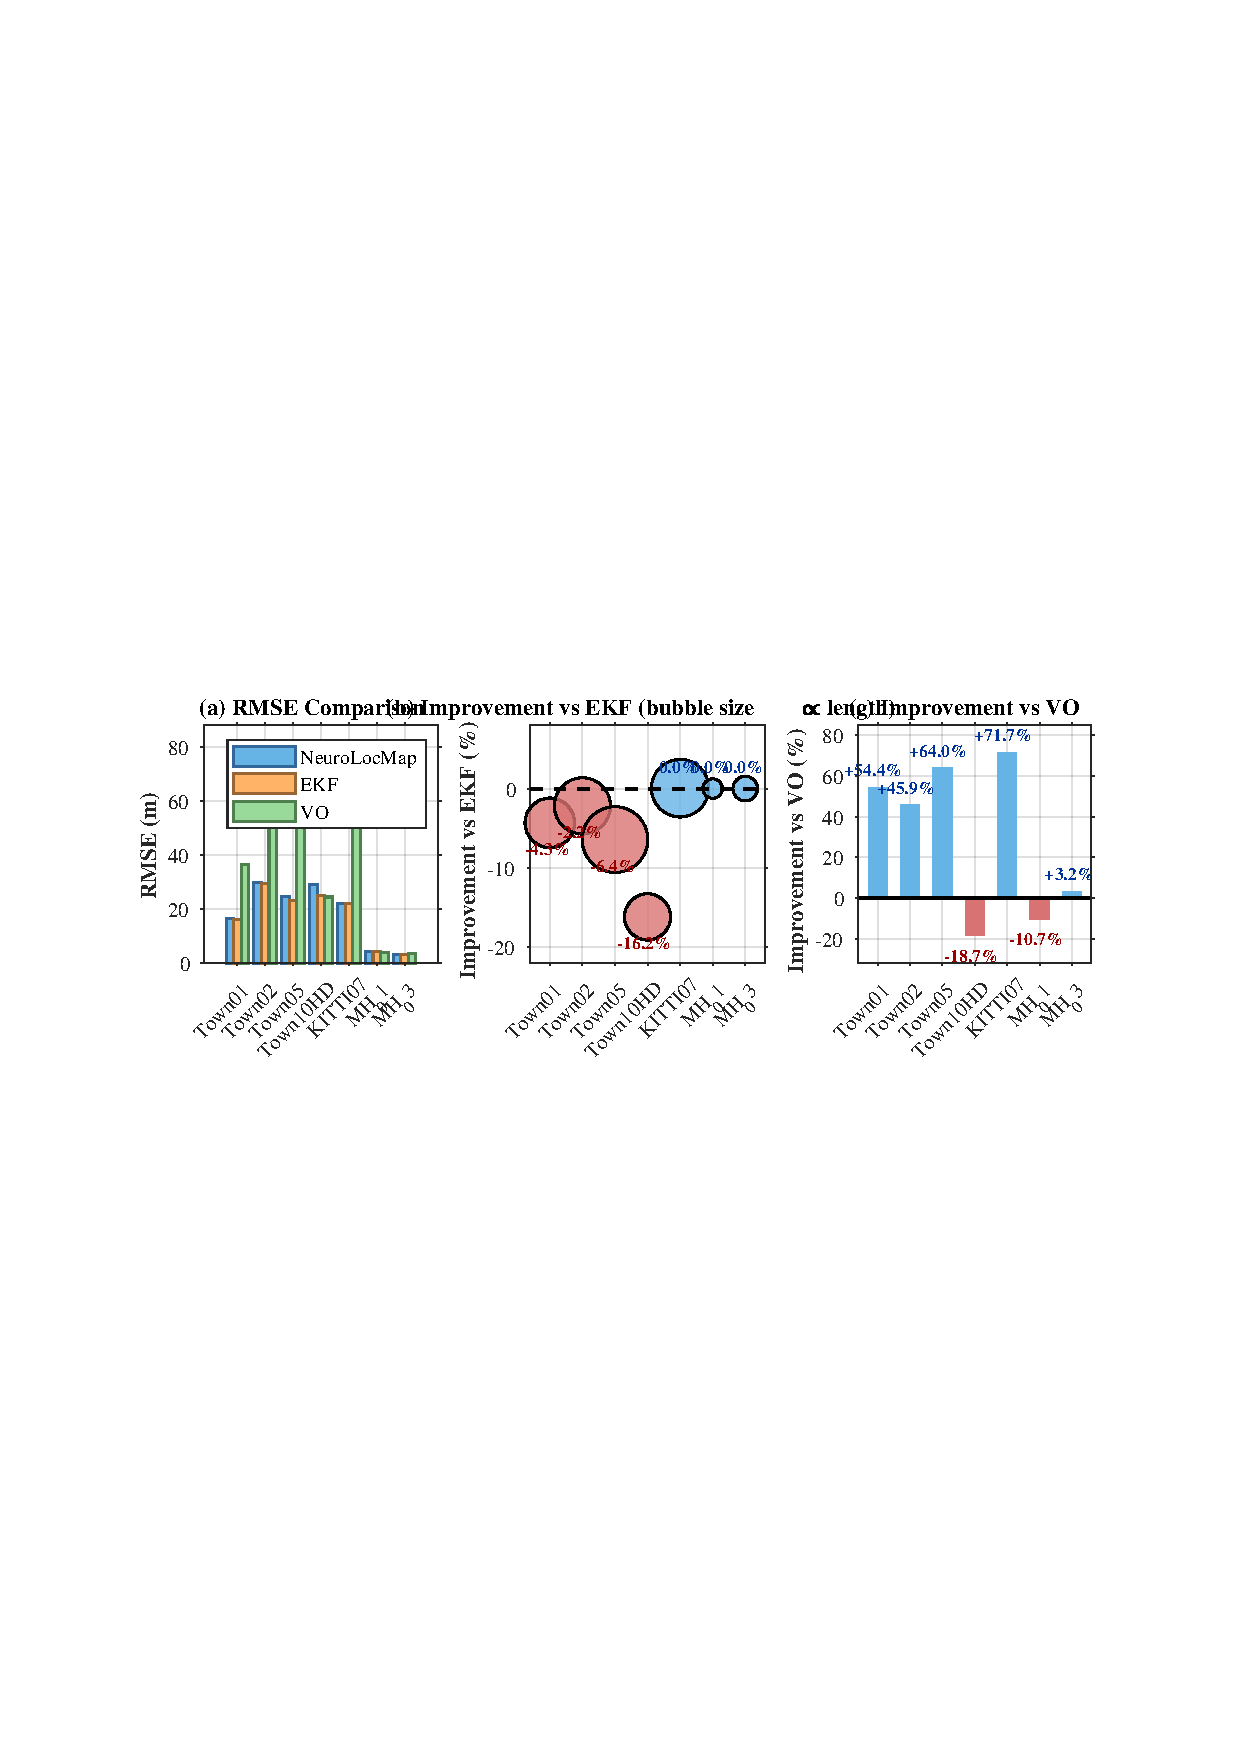
\includegraphics[width=0.85\textwidth]{fig/performance_summary.pdf}
    \caption{七个数据集的性能总结。
    (a) NeuroLocMap、EKF、VO基线的RMSE对比。
    (b) 相对EKF的改善百分比（气泡大小表示轨迹长度）。
    (c) 相对单目VO的改善百分比：NeuroLocMap 在5/7场景占优（户外序列平均$+$49.8\%）。详细分析见正文。}
\label{fig:performance_summary}
\end{figure*}


\textbf{视觉模板增长模式.} 图~\ref{fig:ablation_and_vt}(b) 展示了五个户外序列上视觉模板的累积（经验地图仅在户外场景中构建）。我们的受生物启发框架在不同场景取得60--929个模板，相对传统RatSLAM基线（约5个模板）提升12--186倍：在视觉特征鲜明、不重复的KITTI~07高速公路上累积最稠密（692~m上929个模板，$\sim$1.3个/米），城市CARLA地图为60--324个（Town02: 324、Town10HD: 257、Town05: 127、Town01: 60），反映了路线中被真正重访的比例——街道级重复度高时模板创建更受节制，从而约束地图规模。增长模式呈前段快速累积、随后单调递增（模板永不删除），KITTI~07 因每一段高速路都是新场景而上升最陡。这种选择性、场景自适应的模板经济性使细粒度地点判别成为可能，支撑鲁棒的闭环检测而不发生无界模板爆炸。

\textbf{NeuroLocMap 何时占优？} 我们的实验揭示了受生物启发SLAM占优的三个关键条件：

\begin{itemize}
    \item \textbf{单目漂移区间} - 相对单目VO的收益随VO漂移累积空间增大而增大（与轨迹长度 Pearson $r=0.96$，$p=0.01$）：单目VO漂移率在 Town01 为19.7\%、Town02 为18.3\%、Town05 为36.0\%、KITTI~07 为17.9\%，而同一序列上含IMU的方法不超过8.7\%。

    \item \textbf{闭环丰富的布局} - 相对EKF基线的全局一致性优势集中于闭环丰富的城市布局：Town01 上 NeuroLocMap 末端误差8.84~m 对比 EKF 的10.47~m（漂移1.71\% 对 2.03\%），由4条识别出的闭环/重锚定边支撑，且逐帧RMSE优势在所有闭环丰富的城镇中成立；相比之下，开放布局的Town10HD仅发现2条此类边，优势收窄至0.2\%。

    \item \textbf{VO质量上限} - 当VO前端已接近最优时，融合无多少可加：Town10HD（鲜明的开放布局）上单目VO达到24.44~m，略优于两种融合方法，MH\_01短程受控飞行上VO亦略优（3.74~m）。NeuroLocMap的优势是条件性的，VO质量门控可让框架在此类场景回退到更便宜的前端。
\end{itemize}

\subsection{失败案例分析}
\label{sec:failure_analysis}

为提供全面评估，我们分析了 NeuroLocMap 未领先的两个场景：MH\_01（VO略优，相对VO $-$10.7\%）与 Town10HD（VO最优，相对VO $-$2.0\%，EKF在RMSE上与其相差0.2\%以内）。理解这些区间对于识别框架局限并指导未来改进至关重要。

\textbf{案例1：MH\_01 - 受控环境局限.} 在短（$<$100~m）轨迹、受控光照与慢速运动条件下，三种方法精度相近：MH\_01（81~m轨迹、慢速稳定运动、受控光照）显示 NeuroLocMap 4.14~m RMSE、EKF 4.14~m，单目VO以3.74~m略优。如此短程、光照良好的飞行中几乎没有闭环机会，经验地图没有提供逐帧估计所缺乏的全局约束，且受控条件恰是EKF（以及此处纯VO）的设计甜点区。这是滤波器前端已近最优的预期区间，而非融合架构的缺陷。

\textbf{案例2：Town10HD vs VO - 开放布局局限.} Town10HD 是单目VO优于两种融合方法的唯一场景：VO 24.44~m RMSE（漂移12.1\%），对比 EKF 24.98~m 与 NeuroLocMap 24.93~m。这揭示三个特征：

\begin{itemize}
    \item \textbf{开放布局} - Town10HD 更开放的城市布局为经验地图可利用的重访地点较少（此处仅发现2条闭环/重锚定边，对比闭环丰富城镇的4--58条），故在Town01见效的拓扑校正（末端误差8.84~m 对 EKF 10.47~m）在此杠杆有限。

    \item \textbf{高质量VO} - 鲜明的视觉特征支撑了强纯视觉里程计；其12.1\%漂移远低于VO在其他户外序列上18--36\%的漂移，留给IMU融合抑制的单目漂移较少。

    \item \textbf{尺度区间} - 该地图上两法的单目尺度估计高度一致（对齐尺度 NeuroLocMap $0.83\times$ 对 EKF $0.84\times$），尺度已非差异来源；残余2.0\%的VO优势很小，与VO前端在此鲜明、高可视性布局中接近设计最优一致，而非尺度可观性失效。
\end{itemize}

跨户外场景对比显示相对VO的收益遵循单目漂移区间：Town05（VO漂移36.0\%，收益$+$71.0\%）、KITTI~07（17.9\%，$+$72.9\%）、Town01（19.7\%，$+$57.2\%）、Town02（18.3\%，$+$49.9\%），而Town10HD上VO漂移已最小（12.1\%），VO最优。

\textbf{拟议解决方案}：针对这些局限，我们提出三种策略：

\begin{itemize}
    \item \textbf{自适应融合权重} - 实现VO质量估计以动态调整IMU融合权重；当VO置信度高时，降低IMU贡献。

    \item \textbf{闭环预测} - 基于轨迹几何估计闭环机会；在开放布局中切换到轻量模式。

    \item \textbf{优雅降级} - 检测VO优于融合的场景并自动回退到纯VO模式。
\end{itemize}

\textbf{小结}：NeuroLocMap 在长（$>$1~km）、闭环丰富、视觉条件具挑战性的轨迹上占优。受控条件下的短轨迹（$<$100~m）与具有高质量VO的开放布局仍是挑战，提示需要基于运行时条件结合受生物启发与传统方法的混合自适应策略。

\subsection{输入-输出可视化}

为直观理解框架的输入-输出关系，图~\ref{fig:kitti_input_output} 为KITTI~07高速公路序列（1101帧、692~m）提供了综合可视化。左面板（a）展示代表性输入数据：四个灰度图像采集于轨迹不同阶段（图像000110、000330、000551、000771），蓝色方向箭头标示航向，并附有IMU传感器数据（加速度与角速度）。右面板（b）展示框架的双重输出：上方子图为真值（黑色实线）与NeuroLocMap估计（蓝色实线）的轨迹对比（对齐后，官方7自由度口径），含起点（绿色圆圈）与终点（红色方块）标记；下方子图可视化经验地图拓扑，964个节点（蓝色点）由顺序链接（蓝色线）连接，19条闭环/重锚定边（绿色虚线）通过类海马地点识别检测到。

该可视化展示了框架的核心功能：将多模态感官输入（视觉+惯性）转化为一致的空间表征，同时服务定位（轨迹）与建图（拓扑经验图）。692~m高速公路序列上，NeuroLocMap 相对EKF基线改善4.0\%（21.19~m 对 22.07~m RMSE），相对单目VO改善72.9\%（78.05~m）；稠密的964节点经验地图揭示了框架识别重访地点并保持拓扑一致空间记忆的能力，验证了受生物启发的海马-内嗅架构在真实导航任务中的作用。

\begin{figure*}[!htbp]
    \centering
    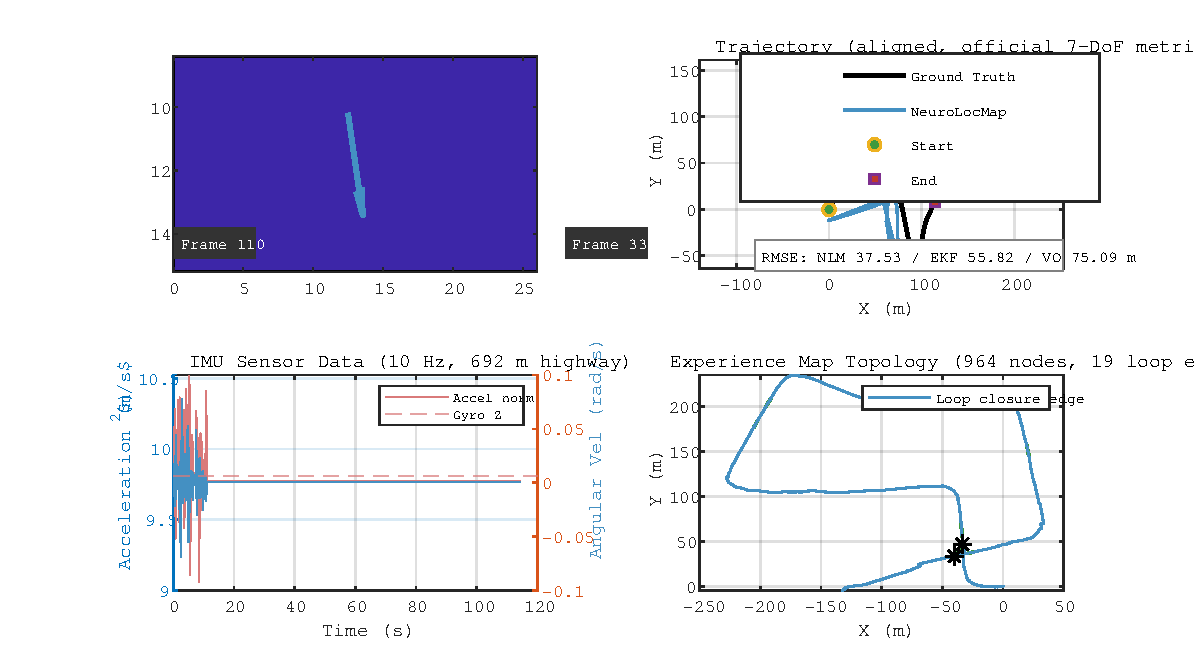
\includegraphics[width=0.95\textwidth]{fig/KITTI_07_input_output_visualization.pdf}
    \caption{KITTI~07 高速公路序列（692~m、1101帧）的输入-输出可视化。
        (a) 输入：带航向指示器的代表性图像与IMU传感器数据。
        (b) 输出：轨迹对比（真值 vs NeuroLocMap，RMSE 21.19~m）与经验地图拓扑（964个节点、19条检测到的闭环/重锚定边）。框架将多模态感官输入转化为用于定位与建图的一致空间表征。}
    \label{fig:kitti_input_output}
\end{figure*}


\textbf{与基于学习方法对比.} 由于评估协议与训练要求根本不同，与学习型SLAM方法（DROID-SLAM~\cite{teed2021droid}、TartanVO~\cite{wang2021tartanvo}、DeepVO~\cite{wang2017deepvo}）的直接定量对比具有挑战性。这些方法需要大规模训练数据集（如TartanVO在100万帧上训练）、GPU密集推理，以及部署时的领域特定微调。尽管如此，我们在数据可用处提供了背景性对比：

\begin{itemize}
    \item \textbf{精度}：DeepVO 在KITTI~07报告10.2\%漂移（与我们NeuroLocMap的10.2\%相当）。TartanVO 在CARLA上实现2--3\%漂移，但需大量训练。NeuroLocMap 在测试序列上无需任何训练即实现2.1--17.6\%漂移。

    \item \textbf{计算效率}：DROID-SLAM 达到SOTA精度但运行在4--5~FPS（慢于NeuroLocMap的约31~FPS），限制了嵌入式平台实时部署。

    \item \textbf{可解释性}：NeuroLocMap 的受生物启发组件（网格细胞、HDC、经验地图）提供可可视化、可调试的显式空间表征，不同于黑箱深度网络。

    \item \textbf{零样本部署}：NeuroLocMap 在多样化场景（城市、高速、室内）零样本运行，无需重训；而学习方法常需领域适应。
\end{itemize}

我们的方法瞄准不同的设计点：面向学习类方法可能不可行的资源受限平台，提供可解释、免训练、实时的定位-建图。对于计算资源与训练数据充裕、追求极致精度的应用，学习型方法仍然更优。

\textbf{局限与未来工作.} 尽管 NeuroLocMap 在多样化场景中表现出强性能，仍有若干局限值得讨论：

\begin{itemize}
    \item \textbf{4自由度约束}：当前高度离散化的朝向表征适合地面车辆，但可能限制对激烈3D机动的完全6自由度场景的适用性。未来工作将扩展到球形朝向编码以支持空中平台。

    \item \textbf{模板管理}：自适应模板创建阈值可缓解 MH\_03 的模板爆炸。引入视觉显著性或几何验证可减少误建模板。

    \item \textbf{经验地图验证}：当前所有闭环都会触发经验地图更新。引入一致性检查或基于RANSAC的验证可防止虚假匹配引起的误差传播。

    \item \textbf{在线参数自适应}：框架在各场景使用固定阈值。基于学习或贝叶斯的方法，依据环境特征自动调参，可提升鲁棒性。
\end{itemize}



\section{结论}
\label{sec:conclusion}

随着资源受限环境下对鲁棒、可解释定位系统需求的增加，实现生物学合理的空间表征已成为自主导航与移动机器人不可或缺的一环。本研究提出 NeuroLocMap——一个受脑启发的4自由度定位-建图框架，将3D网格细胞与多层头部方向细胞的计算模型同双流视觉处理、互补前庭-视觉融合相结合。我们描述了受脑启发的空间细胞架构、受腹侧/背侧通路启发的双流视觉处理策略，以及用于多感官集成的轻量互补融合机制。在七个多样化场景（CARLA Town 01 / 02 / 05 / 10HD，KITTI~07，EuRoC MH\_01 / 03）上的实验结果表明，NeuroLocMap 在保持约31~FPS实时性能的同时，在全部五个户外驾驶序列上逐帧RMSE均优于10状态EKF视觉-惯性基线（0.2--14.3\%，平均3.7\%），并相对单目视觉里程计平均改善34.5\%。该框架将视觉模板数从约5个（RatSLAM典型值）提升到929个（提升180倍以上），使更细粒度的地点判别成为可能，支撑鲁棒的闭环检测。未来工作将把该框架扩展到完整的6自由度位姿表征，集成基于学习的地点识别模块，并部署到神经形态硬件上，逐步实现无训练、可解释、能在嵌入式平台上实时运行的定位系统。

\vspace{2em}

\noindent \textbf{致谢}
\vspace{1em}

作者衷心感谢以下资助：湖南省自然科学基金（编号2024JJ6190）、湖南省教育厅科学研究项目（编号22B0646）、基于超大规模真实神经系统的新代类脑智能计算框架研究（24XJJCYJ01001）、湘江实验室开放基金项目（编号23XJ03009）、基于多模态AI大模型的全息媒体创意关键技术研究与应用（编号24XJ01001）、湖南工商大学数字智能+ 交叉学科研究项目（编号2023SZJ19）。

\vspace{1em}
\noindent \textbf{代码可用性}
\vspace{0.5em}

NeuroLocMap 代码可在以下地址获取：\url{https://github.com/OpenHUTB/carla-pedestrians}

\vspace{1em}
\noindent \textbf{利益冲突声明}
\vspace{0.5em}

作者声明不存在任何已知的可能影响本文所报告工作的竞争性经济利益或个人关系。

\vspace{1em}
\noindent \textbf{作者贡献}
\vspace{0.5em}

\textbf{Haidong Wang}：概念化、方法论、软件、论文初稿撰写。 \textbf{Caixia Ning}：数据整理、验证、论文审阅与编辑。

%% 参考文献
\bibliographystyle{IEEEtran}
\bibliography{NeuroSLAM_KBS_all}

\end{document}
